
\subsection{Analisi Nomi-Verbi}
Viene qui rappresentato l’elenco delle funzionalità che il sistema deve avere, sulla base dal Documento di Visione.
Inoltre, sono presenti le definizioni necessarie.
La legenda spiega come interpretare le informazioni.

\subsubsection{Legenda}

\begin{itemize}
    \item Nomi propri: istanze;
    \item Nomi comuni o predicati nominali: \textcolor{red}{classi} o \textcolor{orange}{attributi};
    %\item \textcolor{teal}{Verbi transitivi}: metodi;
    \item \textcolor{teal}{Verbi}: metodi;
    \item \textcolor{cyan}{Verbi modali}: precondizioni, postcondizioni, o condizioni di invarianza;
    %\item \textcolor{blue}{Verbi intransitivi}: eccezioni o eventi dipendenti dal tempo;
    \item \textcolor{violet}{Aggettivi}: valore di attributo o classe;
    \item  \underline{Riferimenti} alle definizioni.
\end{itemize}

\subsubsection{Definizioni}
\begin{enumerate}
    \item \textcolor{red}{Utente del sistema}: fornito di informazioni riguardanti \textcolor{orange}{nome}, \textcolor{orange}{cognome},
    \textcolor{orange}{data di nascita}, \textcolor{orange}{email}, \textcolor{orange}{password}, \textcolor{orange}{metodi di pagamento}
    Ha la possibilità di sottoscrivere \textcolor{red}{abbonamenti}. Un \textcolor{red}{partner} è un \textcolor{red}{utente} con un \textcolor{red}{abbonamento} che gli consente di pubblicare sulla piattaforma;
    \item \textcolor{red}{Piano di abbonamento}: selezionabile dagli utenti, ha proprietà quali \textcolor{orange}{nome},
    \textcolor{orange}{prezzo}, \textcolor{orange}{durata}, \textcolor{orange}{disponibilità di sottoscrizione}.
    Esso raggruppa una lista di \textcolor{red}{servizi} \textcolor{teal}{offerti};
    \item \textcolor{red}{Servizio}: caratterizzato da \textcolor{orange}{ID} e \textcolor{orange}{descrizione};
    \item \textcolor{red}{Prodotto multimediale}: oltre agli elementi identificativi, è caratterizzato da\textcolor{orange}{genere},
    \textcolor{orange}{visibilità}, \textcolor{red}{utente} \textcolor{orange}{proprietario}. Esso può essere di tipo
    \textcolor{red}{video} o \textcolor{red}{audio}: nel primo caso è fornito di \textcolor{orange}{traccia audio} e
    \textcolor{orange}{traccia video}, nel secondo solo \textcolor{orange}{traccia audio}, ma con accompagnamento di
    \textcolor{orange}{lyrics} o \textcolor{orange}{video musicale};
    \item \textcolor{red}{Playlist}: contenente una lista di \textcolor{red}{prodotti multimediali}.\\
    Casi particolari di essa sono:
    \begin{enumerate}
        \item \textcolor{red}{Serie TV}: formata solamente da \textcolor{violet}{prodotti video}, tutti pubblicati dallo stesso \textcolor{red}{utente};
        \item \textcolor{red}{Album}: formato solamente da \textcolor{violet}{prodotti audio}, tutti pubblicati dallo stesso \textcolor{red}{utente};
    \end{enumerate}
    \item \textcolor{red}{Visualizzazione}: proveniente da un \textcolor{red}{utente} verso un \textcolor{red}{prodotto multimediale},
    considera anche l'\textcolor{orange}{istante} in cui avviene;
    \item \textcolor{red}{Segnalazione}: relativa ad un \textcolor{red}{prodotto multimediale}, caratterizzata dall' \textcolor{red}{utente} che 
    la effettua e una \textcolor{orange}{motivazione};
    \item \textcolor{red}{Coda di riproduzione}: relativa ad un singolo \textcolor{red}{utente}, composta da una lista di  
    \textcolor{red}{prodotti multimediali};
    \item \textcolor{red}{Amministratore del sistema}: \textcolor{teal}{si occupa} della gestione del sistema;
    \item \textcolor{red}{Valutazione}: relative a contenuti e \textcolor{teal}{create} da \textcolor{red}{utenti};
\end{enumerate}

\subsubsection{Funzionalità}
\begin{enumerate}
    \item L' \textcolor{red}{amministratore} \textcolor{teal}{effettua} diverse operazioni sugli \textcolor{red}{abbonamenti}.
    Egli \textcolor{teal}{crea} \textcolor{red}{abbonamenti} e \textcolor{cyan}{può} \textcolor{teal}{attivare} e
    \textcolor{teal}{disattivare} alcuni già \textcolor{violet}{creati}, \textcolor{teal}{modificando} la loro \textcolor{orange}{disponibilità}.
    Inoltre, egli \textcolor{teal}{aggiunge} e \textcolor{teal}{rimuove} \textcolor{red}{servizi} da \textcolor{red}{abbonamenti}.
    L' \textcolor{red}{amministratore} \textcolor{cyan}{può} anche \textcolor{teal}{recuperare} \textcolor{orange}{informazioni} riguardanti
    \textcolor{red}{servizi} (\textcolor{violet}{generici} o in un particolare \textcolor{red}{abbonamento}) e \textcolor{red}{piani di abbonamento};
    \item Il sistema \textcolor{teal}{effettua} pagamenti verso i \textcolor{red}{partner}.
    \item L' \textcolor{red}{amministratore} \textcolor{cyan}{può} \textcolor{teal}{sospendere} l'account di un \textcolor{red}{utente};
    \item L' \textcolor{red}{utente} \textcolor{teal}{effettua} operazioni sul proprio account. Egli \textcolor{teal}{si registra},
    \textcolor{teal}{fornendo} i propri dati, \textcolor{teal}{modifica} il proprio profilo ed \textcolor{teal}{effettua}
    login e logout per \textcolor{teal}{autenticarsi} sulla piattaforma.
    \item L' \textcolor{red}{utente} \textcolor{teal}{richiede} ricerche al sistema. Queste sono relative
    ad un particolare contenuto (\textcolor{red}{prodotto} o \textcolor{red}{playlist}) oppure indirizzate a contenuti
    \textcolor{violet}{popolari}. Inoltre, il sistema \textcolor{teal}{suggerisci} contenuti agli
    \textcolor{red}{utenti}, sulla base delle loro \textcolor{orange}{preferenze};
    \item L' \textcolor{red}{utente} \textcolor{teal}{sottoscrive} nuovi \textcolor{red}{abbonamenti} e ne \textcolor{teal}{disdice} di già
    \textcolor{orange}{sottoscritti}. Egli \textcolor{cyan}{può} \textcolor{teal}{cambiare} un \textcolor{red}{abbonamento} con un altro,
    pagando eventualmente un sovrapprezzo. Il sistema \textcolor{teal}{gestisce} il rinnovo automatico;
    \item Il \textcolor{red}{partner} \textcolor{teal}{pubblica} nuovi \textcolor{red}{prodotti} sulla piattaforma. Egli \textcolor{teal}{compila}
    le \textcolor{orange}{informazioni di base}. Inoltre, nel caso di un 
    \textcolor{red}{prodotto video}, egli \textcolor{teal}{carica} il file video, il file audio e \textcolor{violet}{opzionalmente} sottotitoli.
    Invece, per un \textcolor{red}{prodotto audio}, egli \textcolor{teal}{carica} il file audio e \textcolor{violet}{opzionalmente} video musicale o lyrics.
    Egli, \textcolor{cyan}{può} anche \textcolor{teal}{cambiare} lo stato della pubblicazione, tra \textcolor{violet}{pubblico} e \textcolor{violet}{privato};
    \item L' \textcolor{red}{utente} \textcolor{teal}{riproduce} \textcolor{red}{prodotti} (sia video che audio) con il player. Egli \textcolor{cyan}{può} \textcolor{teal}{mettere}
    il player \textcolor{violet}{in pausa} e \textcolor{violet}{in riproduzione} e \textcolor{teal}{spostare} il punto di riproduzione. 
    Egli \textcolor{cyan}{può} anche \textcolor{teal}{riprodurre} audio in background;
    \item L' \textcolor{red}{utente} \textcolor{teal}{effettua} operazioni sulle \textcolor{red}{playlist}. Egli crea nuove \textcolor{red}{playlist}, \textcolor{violet}{vuote};
    \textcolor{teal}{aggiunge} e \textcolor{teal}{rimuove} \textcolor{red}{prodotti} ad/da esse;  \textcolor{teal}{cambia} la loro \textcolor{orange}{visibilità} (\textcolor{violet}{pubblica} o \textcolor{violet}{privata});
    \textcolor{teal}{riproduce} playlist, che \textcolor{cyan}{devono}  \textcolor{teal}{contenere} almeno un  \textcolor{red}{prodotto};
    \item Il \textcolor{red}{partner} \textcolor{teal}{crea} una \textcolor{red}{serie TV};
    \item Il \textcolor{red}{partner} \textcolor{teal}{crea} un \textcolor{red}{album};
    \item L' \textcolor{red}{utente} \textcolor{cyan}{può} \textcolor{teal}{valutare} contenuti. Egli \textcolor{cyan}{può} \textcolor{teal}{votare} il contenuto
    e/o  \textcolor{teal}{commentarlo}. Il commento \textcolor{cyan}{può} \textcolor{teal}{essere eliminato} dallo stesso \textcolor{red}{utente};
    \item L' \textcolor{red}{utente} \textcolor{cyan}{può} \textcolor{teal}{segnalare} \textcolor{red}{prodotti} e l' \textcolor{red}{amministratore} \textcolor{teal}{controllare} le 
    \textcolor{red}{segnalazioni} di un certo \textcolor{red}{utente};
    \item L' \textcolor{red}{utente} \textcolor{teal}{ottiene} la cronologia dei contenuti visualizzati;
    \item L' \textcolor{red}{utente} \textcolor{teal}{effettua} il download di un certo \textcolor{red}{prodotto};
    \item L' \textcolor{red}{utente} \textcolor{teal}{riproduce} spot pubblicitari.
    \item Il sistema \textcolor{teal}{calcola} il voto di un certo contenuto, sulla base dei voti ricevuti.
    \item L' \textcolor{red}{utente} \textcolor{teal}{effettua} operazioni sulla \textcolor{red}{coda di riproduzione}. Egli \textcolor{teal}{aggiunge}
    e \textcolor{teal}{rimuove} \textcolor{red}{prodotti} da essa. Inoltre, egli \textcolor{cyan}{può} \textcolor{teal}{visualizzare} i 
    \textcolor{red}{prodotti} presenti nella \textcolor{red}{coda}.
\end{enumerate}


%============================ SCHEDE CRC =====================================

\subsection{Schede CRC - Class-Responsability-Collaboration}

Le schede CRC (o card) vengono utilizzate per guidare lo sviluppo orientato agli oggetti del progetto.
con le seguenti schede identifichiamo i principali oggetti e ne specifichiamo per ognuno:
\begin{enumerate}[label=-]
    \item Nome
   \item Superclasse e sottoclassi
    \item gli attributi di cui necessita
    \item le azione che permettera di svolgere
    \item per ogni azione di cui è responsabile verrà specificato
    \begin{enumerate}[label=-]
        \item il Nome
        \item le classi con cui collabora per completare l'azione
   \end{enumerate}
\end{enumerate}

Le basi per la scelta delle classi derivano principalente dall'anailisi dei requisitii (analisi nomi-verbi), con l'aggiunta di alcune classi utili a strutturare meglio il sistema.\\

% ============================ PACKAGE GESTIONE ABBONAMENTI =========================== %
\begin{center}
    \begin{longtable}{ |p{3cm}|p{3cm}|p{3cm}|p{3cm}| }
        \hline
        Nome & \multicolumn{3}{|p{9cm}|}{PianoDiAbbonamento} \\\hline
        Descrizione & \multicolumn{3}{|p{9cm}|}{Classe che rappresenta un piano di abbonamento sottoscrivibile da un utente} \\\hline
        SuperClassi & \multicolumn{3}{|p{9cm}|}{-} \\\hline
        SottoClassi & \multicolumn{3}{|p{9cm}|}{-} \\\hline
        Attributi & \multicolumn{3}{|p{9cm}|}{nome, prezzo, durata, visibilità, lista di servizi offerti} \\\hline
        \multicolumn{4}{|p{12cm}|}{Responsabilit\'a} \\\hline
        \multicolumn{2}{|p{6cm}|}{Nome} & \multicolumn{2}{|p{6cm}|}{Collaboratore} \\\hline
        \multicolumn{2}{|p{6cm}|}{-} & \multicolumn{2}{|p{6cm}|}{-} \\\hline
    \end{longtable}
\end{center}

\begin{center}
    \begin{longtable}{ |p{3cm}|p{3cm}|p{3cm}|p{3cm}| }
        \hline
        Nome & \multicolumn{3}{|p{9cm}|}{SottoscrizioneAbbonamento} \\\hline
        Descrizione & \multicolumn{3}{|p{9cm}|}{Classe che rappresenta un piano di abbonamento sottoscritto da un utente} \\\hline
        SuperClassi & \multicolumn{3}{|p{9cm}|}{-} \\\hline
        SottoClassi & \multicolumn{3}{|p{9cm}|}{-} \\\hline
        Attributi & \multicolumn{3}{|p{9cm}|}{piano di abbonamento, account, data sottoscrizione, rinnovo automatico} \\\hline
        \multicolumn{4}{|p{12cm}|}{Responsabilit\'a} \\\hline
        \multicolumn{2}{|p{6cm}|}{Nome} & \multicolumn{2}{|p{6cm}|}{Collaboratore} \\\hline
        \multicolumn{2}{|p{6cm}|}{-} & \multicolumn{2}{|p{6cm}|}{-} \\\hline
    \end{longtable}
\end{center}

\begin{center}
    \begin{longtable}{ |p{3cm}|p{3cm}|p{3cm}|p{3cm}| }
        \hline
        Nome & \multicolumn{3}{|p{9cm}|}{Servizio} \\\hline
        Descrizione & \multicolumn{3}{|p{9cm}|}{Classe che rappresenta i servizi che possono essere offerti dai vari piani di abbonamento} \\\hline
        SuperClassi & \multicolumn{3}{|p{9cm}|}{-} \\\hline
        SottoClassi & \multicolumn{3}{|p{9cm}|}{-} \\\hline
        Attributi & \multicolumn{3}{|p{9cm}|}{ID, descrizione} \\\hline
        \multicolumn{4}{|p{12cm}|}{Responsabilit\'a} \\\hline
        \multicolumn{2}{|p{6cm}|}{Nome} & \multicolumn{2}{|p{6cm}|}{Collaboratore} \\\hline
        \multicolumn{2}{|p{6cm}|}{-} & \multicolumn{2}{|p{6cm}|}{-} \\\hline
    \end{longtable}
\end{center}

\begin{center}
    \begin{longtable}{ |p{3cm}|p{3cm}|p{3cm}|p{3cm}| }
        \hline
        Nome & \multicolumn{3}{|p{9cm}|}{StoricoPagamento} \\\hline
        Descrizione & \multicolumn{3}{|p{9cm}|}{Classe che rappresenta lo storico di tutte le transazioni di denaro avvenute} \\\hline
        SuperClassi & \multicolumn{3}{|p{9cm}|}{-} \\\hline
        SottoClassi & \multicolumn{3}{|p{9cm}|}{-} \\\hline
        Attributi & \multicolumn{3}{|p{9cm}|}{utente, data emissione, somma traferita, causale, (ricevuto/erogato)} \\\hline
        \multicolumn{4}{|p{12cm}|}{Responsabilit\'a} \\\hline
        \multicolumn{2}{|p{6cm}|}{Nome} & \multicolumn{2}{|p{6cm}|}{Collaboratore} \\\hline
        \multicolumn{2}{|p{6cm}|}{-} & \multicolumn{2}{|p{6cm}|}{-} \\\hline
    \end{longtable}
\end{center}

\begin{center}
    \begin{longtable}{ |p{3cm}|p{3cm}|p{3cm}|p{3cm}| }
        \hline
        Nome & \multicolumn{3}{|p{9cm}|}{HandlerPianoDiAbbonamento} \\\hline
        Descrizione & \multicolumn{3}{|p{9cm}|}{Classe che gestisce le operazioni che possono essere fatte su un piano di abbonamento} \\\hline
        SuperClassi & \multicolumn{3}{|p{9cm}|}{-} \\\hline
        SottoClassi & \multicolumn{3}{|p{9cm}|}{-} \\\hline
        Attributi & \multicolumn{3}{|p{9cm}|}{-} \\\hline
        \multicolumn{4}{|p{12cm}|}{Responsabilit\'a} \\\hline
        \multicolumn{2}{|p{6cm}|}{Nome} & \multicolumn{2}{|p{6cm}|}{Collaboratore} \\\hline
        \multicolumn{2}{|p{6cm}|}{Valida l'input} & \multicolumn{2}{|p{6cm}|}{-} \\\hline
        \multicolumn{2}{|p{6cm}|}{Verifica la presenza di un piano di abbonamento con quel nome} & \multicolumn{2}{|p{6cm}|}{PianoDiAbbonamento} \\\hline
        \multicolumn{2}{|p{6cm}|}{Crea un nuovo piano di abbonamento} & \multicolumn{2}{|p{6cm}|}{PianoDiAbbonamento} \\\hline
        \multicolumn{2}{|p{6cm}|}{Modifica la visibilità del piano di abbonamento} & \multicolumn{2}{|p{6cm}|}{PianoDiAbbonamento} \\\hline
        \multicolumn{2}{|p{6cm}|}{Aggiunge un servizio tra quelli offerti dal piano di abbonamento} & \multicolumn{2}{|p{6cm}|}{PianoDiAbbonamento, Servizio} \\\hline
        \multicolumn{2}{|p{6cm}|}{Rimuove il servizio da quelli offerti dal piano di abbonamento} & \multicolumn{2}{|p{6cm}|}{PianoDiAbbonamento} \\\hline
        \multicolumn{2}{|p{6cm}|}{Cerca i piani di abbonamento sottoscrivibili} & \multicolumn{2}{|p{6cm}|}{PianoDiAbbonamento} \\\hline
    \end{longtable}
\end{center}

\begin{center}
    \begin{longtable}{ |p{3cm}|p{3cm}|p{3cm}|p{3cm}| }
        \hline
        Nome & \multicolumn{3}{|p{9cm}|}{HandlerSottoscrizioneAbbonamento} \\\hline
        Descrizione & \multicolumn{3}{|p{9cm}|}{Classe che gestisce le operazioni che possono essere fatte su una sottoscrizione di piano di abbonamento} \\\hline
        SuperClassi & \multicolumn{3}{|p{9cm}|}{-} \\\hline
        SottoClassi & \multicolumn{3}{|p{9cm}|}{-} \\\hline
        Attributi & \multicolumn{3}{|p{9cm}|}{-} \\\hline
        \multicolumn{4}{|p{12cm}|}{Responsabilit\'a} \\\hline
        \multicolumn{2}{|p{6cm}|}{Nome} & \multicolumn{2}{|p{6cm}|}{Collaboratore} \\\hline
        \multicolumn{2}{|p{6cm}|}{Richiede il pagamento} & \multicolumn{2}{|p{6cm}|}{APIPagamento} \\\hline
        \multicolumn{2}{|p{6cm}|}{Aggiunge il piano di abbonamento tra quelli posseduti dall'utente} & \multicolumn{2}{|p{6cm}|}{SottoscrizioneAbbonamento} \\\hline
        \multicolumn{2}{|p{6cm}|}{Annulla il rinnovo automatico dell'abbonamento} & \multicolumn{2}{|p{6cm}|}{SottoscrizioneAbbonamento} \\\hline
        \multicolumn{2}{|p{6cm}|}{Permette il cambio di un piano di abbonamento con un altro} & \multicolumn{2}{|p{6cm}|}{SottoscrizioneAbbonamento, PianoDiAbbonamento, APIPagamento} \\\hline
        \multicolumn{2}{|p{6cm}|}{Cerca i piani di abbonamento sottoscritti da un utente} & \multicolumn{2}{|p{6cm}|}{SottoscrizioneAbbonamento} \\\hline
    \end{longtable}
\end{center}

\begin{center}
    \begin{longtable}{ |p{3cm}|p{3cm}|p{3cm}|p{3cm}| }
        \hline
        Nome & \multicolumn{3}{|p{9cm}|}{HandlerPagamento} \\\hline
        Descrizione & \multicolumn{3}{|p{9cm}|}{Classe che gestisce i pagamenti sia verso alcuni utenti sia verso il sistema per il rinnovo degli abbonamenti } \\\hline
        SuperClassi & \multicolumn{3}{|p{9cm}|}{-} \\\hline
        SottoClassi & \multicolumn{3}{|p{9cm}|}{-} \\\hline
        Attributi & \multicolumn{3}{|p{9cm}|}{-} \\\hline
        \multicolumn{4}{|p{12cm}|}{Responsabilit\'a} \\\hline
        \multicolumn{2}{|p{6cm}|}{Nome} & \multicolumn{2}{|p{6cm}|}{Collaboratore} \\\hline
        \multicolumn{2}{|p{6cm}|}{Calcola l'importo da pagare} & \multicolumn{2}{|p{6cm}|}{Riproduzione, HandlerRicerche, Prodotto} \\\hline
        \multicolumn{2}{|p{6cm}|}{Effettua il pagamento verso partner} & \multicolumn{2}{|p{6cm}|}{APISistemaPagamento, HandlerSottoscrizioniAbbonamento} \\\hline
        \multicolumn{2}{|p{6cm}|}{Gestisce il rinnovo automatico delle sottoscrizoni ai piani di abbonamento} & \multicolumn{2}{|p{6cm}|}{APISistemaPagamento, HandlerSottoscrizioniAbbonamento} \\\hline
        \multicolumn{2}{|p{6cm}|}{Aggiorna lo storico dei vari pagamenti avvenuti (sia verso l'utente, sia verso il sistema)} & \multicolumn{2}{|p{6cm}|}{StoricoPagamento} \\\hline
    \end{longtable}
\end{center}

\begin{center}
    \begin{longtable}{ |p{3cm}|p{3cm}|p{3cm}|p{3cm}| }
        \hline
        Nome & \multicolumn{3}{|p{9cm}|}{APIPagamento} \\\hline
        Descrizione & \multicolumn{3}{|p{9cm}|}{Classe che gestisce i vari pagamenti da e verso l'utente} \\\hline
        SuperClassi & \multicolumn{3}{|p{9cm}|}{-} \\\hline
        SottoClassi & \multicolumn{3}{|p{9cm}|}{-} \\\hline
        Attributi & \multicolumn{3}{|p{9cm}|}{-} \\\hline
        \multicolumn{4}{|p{12cm}|}{Responsabilit\'a} \\\hline
        \multicolumn{2}{|p{6cm}|}{Nome} & \multicolumn{2}{|p{6cm}|}{Collaboratore} \\\hline
        \multicolumn{2}{|p{6cm}|}{Gestisce il pagamento dei piani di abbonamento} & \multicolumn{2}{|p{6cm}|}{HandlerPagamento} \\\hline
        \multicolumn{2}{|p{6cm}|}{Gestisce il pagamento verso gli utenti partner} & \multicolumn{2}{|p{6cm}|}{HandlerPagamento} \\\hline
    \end{longtable}
\end{center}

\begin{center}
    \begin{longtable}{ |p{3cm}|p{3cm}|p{3cm}|p{3cm}| }
        \hline
        Nome & \multicolumn{3}{|p{9cm}|}{UIGestionePianoDiAbbonamento} \\\hline
        Descrizione & \multicolumn{3}{|p{9cm}|}{Classe che rappresenta l'insieme degli elementi dell'interfaccia che permettono la gestione dei piani di abbonamento da parte dell'amministratore} \\\hline
        SuperClassi & \multicolumn{3}{|p{9cm}|}{-} \\\hline
        SottoClassi & \multicolumn{3}{|p{9cm}|}{-} \\\hline
        Attributi & \multicolumn{3}{|p{9cm}|}{-} \\\hline
        \multicolumn{4}{|p{12cm}|}{Responsabilit\'a} \\\hline
        \multicolumn{2}{|p{5cm}|}{Nome} & \multicolumn{2}{|p{7cm}|}{Collaboratore} \\\hline
        \multicolumn{2}{|p{5cm}|}{Mostra i piani di abbonamento} & \multicolumn{2}{|p{7cm}|}{PianoDiAbbonamento} \\\hline
        \multicolumn{2}{|p{5cm}|}{Invia i dati alle classi di gestione} & \multicolumn{2}{|p{7cm}|}{HandlerPianoDiAbbonamento} \\\hline
        \multicolumn{2}{|p{5cm}|}{Visualizza i messaggi di risposta} & \multicolumn{2}{|p{7cm}|}{HandlerPianoDiAbbonamento} \\\hline
    \end{longtable}
\end{center}

\begin{center}
    \begin{longtable}{ |p{3cm}|p{3cm}|p{3cm}|p{3cm}| }
        \hline
        Nome & \multicolumn{3}{|p{9cm}|}{UIPianoDiAbbonamento} \\\hline
        Descrizione & \multicolumn{3}{|p{9cm}|}{Classe che rappresenta l'insieme degli elementi dell'interfaccia che permettono la gestione dei piani di abbonamento da parte di un utente} \\\hline
        SuperClassi & \multicolumn{3}{|p{9cm}|}{-} \\\hline
        SottoClassi & \multicolumn{3}{|p{9cm}|}{-} \\\hline
        Attributi & \multicolumn{3}{|p{9cm}|}{-} \\\hline
        \multicolumn{4}{|p{12cm}|}{Responsabilit\'a} \\\hline
        \multicolumn{2}{|p{5cm}|}{Nome} & \multicolumn{2}{|p{7cm}|}{Collaboratore} \\\hline
        \multicolumn{2}{|p{5cm}|}{Mostra i piani di abbonamento} & \multicolumn{2}{|p{7cm}|}{HandlerPianoDiAbbonamento} \\\hline
        \multicolumn{2}{|p{5cm}|}{Invia i dati alle classi di gestione} & \multicolumn{2}{|p{7cm}|}{HandlerSottoscrizioneAbbonamento} \\\hline
        \multicolumn{2}{|p{5cm}|}{Visualizza i messaggi di risposta} & \multicolumn{2}{|p{7cm}|}{HandlerSottoscrizioneAbbonamento} \\\hline
    \end{longtable}
\end{center}

\begin{center}
    \begin{longtable}{ |p{3cm}|p{3cm}|p{3cm}|p{3cm}| }
        \hline
        Nome & \multicolumn{3}{|p{9cm}|}{UIGestioneSottoscrizioneAbbonamento} \\\hline
        Descrizione & \multicolumn{3}{|p{9cm}|}{Classe che rappresenta l'insieme degli elementi dell'interfaccia che permettono la gestione dei piani di abbonamento sottoscritti da un utente} \\\hline
        SuperClassi & \multicolumn{3}{|p{9cm}|}{-} \\\hline
        SottoClassi & \multicolumn{3}{|p{9cm}|}{-} \\\hline
        Attributi & \multicolumn{3}{|p{9cm}|}{-} \\\hline
        \multicolumn{4}{|p{12cm}|}{Responsabilit\'a} \\\hline
        \multicolumn{2}{|p{5cm}|}{Nome} & \multicolumn{2}{|p{7cm}|}{Collaboratore} \\\hline
        \multicolumn{2}{|p{5cm}|}{Mostra i piani di abbonamento sottoscritti} & \multicolumn{2}{|p{7cm}|}{HandlerSottoscrizioneAbbonamento} \\\hline
        \multicolumn{2}{|p{5cm}|}{Invia i dati alle classi di gestione} & \multicolumn{2}{|p{7cm}|}{HandlerSottoscrizioneAbbonamento} \\\hline
        \multicolumn{2}{|p{5cm}|}{Visualizza i messaggi di risposta} & \multicolumn{2}{|p{7cm}|}{HandlerSottoscrizioneAbbonamento} \\\hline
    \end{longtable}
\end{center}
% ================================================================================= %

% ============================ PACKAGE GESTIONE ACCOUNT =========================== %
\begin{center} % CLASS %
    \begin{longtable}{ |p{3cm}|p{3cm}|p{3cm}|p{3cm}| }
        \hline
        Nome & \multicolumn{3}{|p{9cm}|}{Persona} \\\hline
        Descrizione & \multicolumn{3}{|p{9cm}|}{Memorizza le informazioni anagrafiche e di pagamento/fatturazione di una persona registrata alla piattaforma} \\\hline
        SuperClassi & \multicolumn{3}{|p{9cm}|}{-} \\\hline
        SottoClassi & \multicolumn{3}{|p{9cm}|}{-} \\\hline
        Attributi & \multicolumn{3}{|p{9cm}|}{nome, cognome, data di nascita, dati fatturazione (CoordinateBancarie), lista dati pagamento (lista CoordinateBancarie), riferimento pagamento predefinito} \\\hline
        \multicolumn{4}{|p{12cm}|}{Responsabilit\'a} \\\hline %%% RESPONSABILITA %%%
        \multicolumn{2}{|p{6cm}|}{Nome} & \multicolumn{2}{|p{6cm}|}{Collaboratore} \\\hline %%%%%%%
        \multicolumn{2}{|p{6cm}|}{-} & \multicolumn{2}{|p{6cm}|}{-} \\\hline
    \end{longtable}
\end{center}

\begin{center} % CLASS %
    \begin{longtable}{ |p{3cm}|p{3cm}|p{3cm}|p{3cm}| }
        \hline
        Nome & \multicolumn{3}{|p{9cm}|}{Account} \\\hline
        Descrizione & \multicolumn{3}{|p{9cm}|}{Memorizza le informazioni generiche di un account} \\\hline
        SuperClassi & \multicolumn{3}{|p{9cm}|}{-} \\\hline
        SottoClassi & \multicolumn{3}{|p{9cm}|}{AccountUtente, AccountAmministratore} \\\hline
        Attributi & \multicolumn{3}{|p{9cm}|}{email, email recupero, hash password, data registrazione, proprietario (Persona), data fine blocco} \\\hline
        \multicolumn{4}{|p{12cm}|}{Responsabilit\'a} \\\hline %%% RESPONSABILITA %%%
        \multicolumn{2}{|p{6cm}|}{Nome} & \multicolumn{2}{|p{6cm}|}{Collaboratore} \\\hline %%%%%%%
        \multicolumn{2}{|p{6cm}|}{-} & \multicolumn{2}{|p{6cm}|}{-} \\\hline
    \end{longtable}
\end{center}

\begin{center} % CLASS %
    \begin{longtable}{ |p{3cm}|p{3cm}|p{3cm}|p{3cm}| }
        \hline
        Nome & \multicolumn{3}{|p{9cm}|}{AccountUtente} \\\hline
        Descrizione & \multicolumn{3}{|p{9cm}|}{Memorizza le informazioni rispettive ad un account utente} \\\hline
        SuperClassi & \multicolumn{3}{|p{9cm}|}{Account} \\\hline
        SottoClassi & \multicolumn{3}{|p{9cm}|}{-} \\\hline
        Attributi & \multicolumn{3}{|p{9cm}|}{lista abbonamenti sottoscritti} \\\hline
        \multicolumn{4}{|p{12cm}|}{Responsabilit\'a} \\\hline %%% RESPONSABILITA %%%
        \multicolumn{2}{|p{6cm}|}{Nome} & \multicolumn{2}{|p{6cm}|}{Collaboratore} \\\hline %%%%%%%
        \multicolumn{2}{|p{6cm}|}{-} & \multicolumn{2}{|p{6cm}|}{-} \\\hline
    \end{longtable}
\end{center}

\begin{center} % CLASS %
    \begin{longtable}{ |p{3cm}|p{3cm}|p{3cm}|p{3cm}| }
        \hline
        Nome & \multicolumn{3}{|p{9cm}|}{AccountAmministratore} \\\hline
        Descrizione & \multicolumn{3}{|p{9cm}|}{Memorizza le informazioni rispettive ad un account amministratore} \\\hline
        SuperClassi & \multicolumn{3}{|p{9cm}|}{Account} \\\hline
        SottoClassi & \multicolumn{3}{|p{9cm}|}{-} \\\hline
        Attributi & \multicolumn{3}{|p{9cm}|}{lista permessi} \\\hline
        \multicolumn{4}{|p{12cm}|}{Responsabilit\'a} \\\hline %%% RESPONSABILITA %%%
        \multicolumn{2}{|p{6cm}|}{Nome} & \multicolumn{2}{|p{6cm}|}{Collaboratore} \\\hline %%%%%%%
        \multicolumn{2}{|p{6cm}|}{-} & \multicolumn{2}{|p{6cm}|}{-} \\\hline
    \end{longtable}
\end{center}

\begin{center} % CLASS %
    \begin{longtable}{ |p{3cm}|p{3cm}|p{3cm}|p{3cm}| }
        \hline
        Nome & \multicolumn{3}{|p{9cm}|}{Permesso} \\\hline
        Descrizione & \multicolumn{3}{|p{9cm}|}{Modella i permessi secondo i quali gli amministratori possono o no accedere a determinate parti del sistema} \\\hline
        SuperClassi & \multicolumn{3}{|p{9cm}|}{-} \\\hline
        SottoClassi & \multicolumn{3}{|p{9cm}|}{-} \\\hline
        Attributi & \multicolumn{3}{|p{9cm}|}{nome, descrizione} \\\hline
        \multicolumn{4}{|p{12cm}|}{Responsabilit\'a} \\\hline %%% RESPONSABILITA %%%
        \multicolumn{2}{|p{6cm}|}{Nome} & \multicolumn{2}{|p{6cm}|}{Collaboratore} \\\hline %%%%%%%
        \multicolumn{2}{|p{6cm}|}{-} & \multicolumn{2}{|p{6cm}|}{-} \\\hline
    \end{longtable}
\end{center}

\begin{center} % CLASS %
    \begin{longtable}{ |p{3cm}|p{3cm}|p{3cm}|p{3cm}| }
        \hline
        Nome & \multicolumn{3}{|p{9cm}|}{MetodoDiPagamento} \\\hline
        Descrizione & \multicolumn{3}{|p{9cm}|}{Memorizza i tipi di metodi di pagamento utulizzabili sul sistema} \\\hline
        SuperClassi & \multicolumn{3}{|p{9cm}|}{-} \\\hline
        SottoClassi & \multicolumn{3}{|p{9cm}|}{-} \\\hline
        Attributi & \multicolumn{3}{|p{9cm}|}{nome} \\\hline
        \multicolumn{4}{|p{12cm}|}{Responsabilit\'a} \\\hline %%% RESPONSABILITA %%%
        \multicolumn{2}{|p{6cm}|}{Nome} & \multicolumn{2}{|p{6cm}|}{Collaboratore} \\\hline %%%%%%%
        \multicolumn{2}{|p{6cm}|}{-} & \multicolumn{2}{|p{6cm}|}{-} \\\hline
    \end{longtable}
\end{center}

\begin{center} % CLASS %
    \begin{longtable}{ |p{3cm}|p{3cm}|p{3cm}|p{3cm}| }
        \hline
        Nome & \multicolumn{3}{|p{9cm}|}{CoordinateBancarie} \\\hline
        Descrizione & \multicolumn{3}{|p{9cm}|}{Memorizza le informazioni rispettive alle coordinate bancarie degli utenti} \\\hline
        SuperClassi & \multicolumn{3}{|p{9cm}|}{-} \\\hline
        SottoClassi & \multicolumn{3}{|p{9cm}|}{-} \\\hline
        Attributi & \multicolumn{3}{|p{9cm}|}{codice, tipo di pagamento (MetodoDiPagamento)} \\\hline
        \multicolumn{4}{|p{12cm}|}{Responsabilit\'a} \\\hline %%% RESPONSABILITA %%%
        \multicolumn{2}{|p{6cm}|}{Nome} & \multicolumn{2}{|p{6cm}|}{Collaboratore} \\\hline %%%%%%%
        \multicolumn{2}{|p{6cm}|}{-} & \multicolumn{2}{|p{6cm}|}{-} \\\hline
    \end{longtable}
\end{center}

\begin{center} % UI %
    \begin{longtable}{ |p{3cm}|p{3cm}|p{3cm}|p{3cm}| }
        \hline
        Nome & \multicolumn{3}{|p{9cm}|}{UIUtenteAutenticato} \\\hline
        Descrizione & \multicolumn{3}{|p{9cm}|}{fornisce l'interfaccia agli utenti autenticati} \\\hline
        SuperClassi & \multicolumn{3}{|p{9cm}|}{-} \\\hline
        SottoClassi & \multicolumn{3}{|p{9cm}|}{-} \\\hline
        Attributi & \multicolumn{3}{|p{9cm}|}{-} \\\hline
        \multicolumn{4}{|p{12cm}|}{Responsabilit\'a} \\\hline %%% RESPONSABILITA %%%
        \multicolumn{2}{|p{6cm}|}{Nome} & \multicolumn{2}{|p{6cm}|}{Collaboratore} \\\hline %%%%%%%
        \multicolumn{2}{|p{6cm}|}{Permette la getione dell'utente e l'accesso} & \multicolumn{2}{|p{6cm}|}{HandlerProfiloUtente} \\\hline
        \multicolumn{2}{|p{6cm}|}{Permette di gestire gli abbonamenti sottoscritti} & \multicolumn{2}{|p{6cm}|}{UIGestioneSottoscrizioneAbbonamento} \\\hline
        \multicolumn{2}{|p{6cm}|}{Permette la sottoscrizione di nuovi abbonamenti} & \multicolumn{2}{|p{6cm}|}{UIPianoDiAbbonamento} \\\hline
        \multicolumn{2}{|p{6cm}|}{Permette di visualizzare la cronologia} & \multicolumn{2}{|p{6cm}|}{HandlerCronologia} \\\hline
    \end{longtable}
\end{center}

\begin{center} % UI %
    \begin{longtable}{ |p{3cm}|p{3cm}|p{3cm}|p{3cm}| }
        \hline
        Nome & \multicolumn{3}{|p{9cm}|}{UIUtenteNonAutenticato} \\\hline
        Descrizione & \multicolumn{3}{|p{9cm}|}{fornisce l'interfaccia agli utentei non autenticati} \\\hline
        SuperClassi & \multicolumn{3}{|p{9cm}|}{-} \\\hline
        SottoClassi & \multicolumn{3}{|p{9cm}|}{-} \\\hline
        Attributi & \multicolumn{3}{|p{9cm}|}{-} \\\hline
        \multicolumn{4}{|p{12cm}|}{Responsabilit\'a} \\\hline %%% RESPONSABILITA %%%
        \multicolumn{2}{|p{6cm}|}{Nome} & \multicolumn{2}{|p{6cm}|}{Collaboratore} \\\hline %%%%%%%
        \multicolumn{2}{|p{6cm}|}{Permette il logout dalla piattaforma} & \multicolumn{2}{|p{6cm}|}{HandlerProfiloUtente} \\\hline
        \multicolumn{2}{|p{6cm}|}{Permette la registrazione di nuovi utenti} & \multicolumn{2}{|p{6cm}|}{HandlerProfiloUtente} \\\hline
        
    \end{longtable}
\end{center}

% \begin{center} % UI %
%     \begin{longtable}{ |p{3cm}|p{3cm}|p{3cm}|p{3cm}| }
%         \hline
%         Nome & \multicolumn{3}{|p{9cm}|}{UIAmministratore} \\\hline
%         Descrizione & \multicolumn{3}{|p{9cm}|}{fornisce l'interfaccia per la modifica del profilo di amministratore} \\\hline
%         SuperClassi & \multicolumn{3}{|p{9cm}|}{-} \\\hline
%         SottoClassi & \multicolumn{3}{|p{9cm}|}{-} \\\hline
%         Attributi & \multicolumn{3}{|p{9cm}|}{-} \\\hline
%         \multicolumn{4}{|p{12cm}|}{Responsabilit\'a} \\\hline %%% RESPONSABILITA %%%
%         \multicolumn{2}{|p{6cm}|}{Nome} & \multicolumn{2}{|p{6cm}|}{Collaboratore} \\\hline %%%%%%%
%         \multicolumn{2}{|p{6cm}|}{Permette la modifica delle informazioni dell'amministratore} & \multicolumn{2}{|p{6cm}|}{HandlerAccountAmministratore} \\\hline
        
%     \end{longtable}
% \end{center}

% \begin{center} % UI %
%     \begin{longtable}{ |p{3cm}|p{3cm}|p{3cm}|p{3cm}| }
%         \hline
%         Nome & \multicolumn{3}{|p{9cm}|}{UIPermessi} \\\hline
%         Descrizione & \multicolumn{3}{|p{9cm}|}{fornisce l'interfaccia per la modifica dei permessi di amministrazione} \\\hline
%         SuperClassi & \multicolumn{3}{|p{9cm}|}{-} \\\hline
%         SottoClassi & \multicolumn{3}{|p{9cm}|}{-} \\\hline
%         Attributi & \multicolumn{3}{|p{9cm}|}{-} \\\hline
%         \multicolumn{4}{|p{12cm}|}{Responsabilit\'a} \\\hline %%% RESPONSABILITA %%%
%         \multicolumn{2}{|p{6cm}|}{Nome} & \multicolumn{2}{|p{6cm}|}{Collaboratore} \\\hline %%%%%%%
%         \multicolumn{2}{|p{6cm}|}{Permette la gestione dei permessi} & \multicolumn{2}{|p{6cm}|}{HandlerPermesso} \\\hline
        
%     \end{longtable}
% \end{center}

% \begin{center} % UI %
%     \begin{longtable}{ |p{3cm}|p{3cm}|p{3cm}|p{3cm}| }
%         \hline
%         Nome & \multicolumn{3}{|p{9cm}|}{UIMetodiDiPagamento} \\\hline
%         Descrizione & \multicolumn{3}{|p{9cm}|}{fornisce l'interfaccia per la modifica dei metodi di pagamento} \\\hline
%         SuperClassi & \multicolumn{3}{|p{9cm}|}{-} \\\hline
%         SottoClassi & \multicolumn{3}{|p{9cm}|}{-} \\\hline
%         Attributi & \multicolumn{3}{|p{9cm}|}{-} \\\hline
%         \multicolumn{4}{|p{12cm}|}{Responsabilit\'a} \\\hline %%% RESPONSABILITA %%%
%         \multicolumn{2}{|p{6cm}|}{Nome} & \multicolumn{2}{|p{6cm}|}{Collaboratore} \\\hline %%%%%%%
%         \multicolumn{2}{|p{6cm}|}{Permette la gestione dei metodi di pagamento} & \multicolumn{2}{|p{6cm}|}{HandlerMetodoDiPagamento} \\\hline
        
%     \end{longtable}
% \end{center}

\begin{center} % UI %
    \begin{longtable}{ |p{3cm}|p{3cm}|p{3cm}|p{3cm}| }
        \hline
        Nome & \multicolumn{3}{|p{9cm}|}{UIBan} \\\hline
        Descrizione & \multicolumn{3}{|p{9cm}|}{fornisce l'interfaccia per la gestione degli account bloccati o da bloccare} \\\hline
        SuperClassi & \multicolumn{3}{|p{9cm}|}{-} \\\hline
        SottoClassi & \multicolumn{3}{|p{9cm}|}{-} \\\hline
        Attributi & \multicolumn{3}{|p{9cm}|}{-} \\\hline
        \multicolumn{4}{|p{12cm}|}{Responsabilit\'a} \\\hline %%% RESPONSABILITA %%%
        \multicolumn{2}{|p{6cm}|}{Nome} & \multicolumn{2}{|p{6cm}|}{Collaboratore} \\\hline %%%%%%%
        \multicolumn{2}{|p{6cm}|}{sbloccare un utente bloccato} & \multicolumn{2}{|p{6cm}|}{APIBan} \\\hline        
        \multicolumn{2}{|p{6cm}|}{bloccare un utente} & \multicolumn{2}{|p{6cm}|}{APIBan} \\\hline        
    \end{longtable}
\end{center}

\begin{center} % UI %
    \begin{longtable}{ |p{3cm}|p{3cm}|p{3cm}|p{3cm}| }
        \hline
        Nome & \multicolumn{3}{|p{9cm}|}{APIBan} \\\hline
        Descrizione & \multicolumn{3}{|p{9cm}|}{fornisce l'interfaccia per la gestione degli account bloccati} \\\hline
        SuperClassi & \multicolumn{3}{|p{9cm}|}{-} \\\hline
        SottoClassi & \multicolumn{3}{|p{9cm}|}{-} \\\hline
        Attributi & \multicolumn{3}{|p{9cm}|}{-} \\\hline
        \multicolumn{4}{|p{12cm}|}{Responsabilit\'a} \\\hline %%% RESPONSABILITA %%%
        \multicolumn{2}{|p{6cm}|}{Nome} & \multicolumn{2}{|p{6cm}|}{Collaboratore} \\\hline %%%%%%%
        \multicolumn{2}{|p{6cm}|}{permette di bloccare e sbloccare un utente} & \multicolumn{2}{|p{6cm}|}{HandlerBan} \\\hline        
    \end{longtable}
\end{center}

\begin{center} % HANDLER %
    \begin{longtable}{ |p{3cm}|p{3cm}|p{3cm}|p{3cm}| }
        \hline
        Nome & \multicolumn{3}{|p{9cm}|}{HandlerCronologia} \\\hline
        Descrizione & \multicolumn{3}{|p{9cm}|}{gestisce le operazioni per calcolare e mantenere la cronologia utente} \\\hline
        SuperClassi & \multicolumn{3}{|p{9cm}|}{-} \\\hline
        SottoClassi & \multicolumn{3}{|p{9cm}|}{-} \\\hline
        Attributi & \multicolumn{3}{|p{9cm}|}{-} \\\hline
        \multicolumn{4}{|p{12cm}|}{Responsabilit\'a} \\\hline %%% RESPONSABILITA %%%
        \multicolumn{2}{|p{6cm}|}{Nome} & \multicolumn{2}{|p{6cm}|}{Collaboratore} \\\hline %%%%%%%
        \multicolumn{2}{|p{6cm}|}{mostra la cronologia delle riproduzioni} & \multicolumn{2}{|p{6cm}|}{Riproduzione} \\\hline
        \end{longtable}
\end{center}

% \begin{center} % HANDLER %
%     \begin{longtable}{ |p{3cm}|p{3cm}|p{3cm}|p{3cm}| }
%         \hline
%         Nome & \multicolumn{3}{|p{9cm}|}{HandlerLogout} \\\hline
%         Descrizione & \multicolumn{3}{|p{9cm}|}{gestisce le operazioni per l'accesso e la disconnessione degli utenti} \\\hline
%         SuperClassi & \multicolumn{3}{|p{9cm}|}{-} \\\hline
%         SottoClassi & \multicolumn{3}{|p{9cm}|}{-} \\\hline
%         Attributi & \multicolumn{3}{|p{9cm}|}{-} \\\hline
%         \multicolumn{4}{|p{12cm}|}{Responsabilit\'a} \\\hline %%% RESPONSABILITA %%%
%         \multicolumn{2}{|p{6cm}|}{Nome} & \multicolumn{2}{|p{6cm}|}{Collaboratore} \\\hline %%%%%%%
%         \multicolumn{2}{|p{6cm}|}{effettua logout} & \multicolumn{2}{|p{6cm}|}{-} \\\hline
%         \end{longtable}
% \end{center}

% \begin{center} % HANDLER %
%     \begin{longtable}{ |p{3cm}|p{3cm}|p{3cm}|p{3cm}| }
%         \hline
%         Nome & \multicolumn{3}{|p{9cm}|}{HandlerLogin} \\\hline
%         Descrizione & \multicolumn{3}{|p{9cm}|}{gestisce le operazioni per l'accesso e la disconnessione degli utenti} \\\hline
%         SuperClassi & \multicolumn{3}{|p{9cm}|}{-} \\\hline
%         SottoClassi & \multicolumn{3}{|p{9cm}|}{-} \\\hline
%         Attributi & \multicolumn{3}{|p{9cm}|}{-} \\\hline
%         \multicolumn{4}{|p{12cm}|}{Responsabilit\'a} \\\hline %%% RESPONSABILITA %%%
%         \multicolumn{2}{|p{6cm}|}{Nome} & \multicolumn{2}{|p{6cm}|}{Collaboratore} \\\hline %%%%%%%
%         \multicolumn{2}{|p{6cm}|}{valida credenziali} & \multicolumn{2}{|p{6cm}|}{Account} \\\hline
%         \multicolumn{2}{|p{6cm}|}{effettua login} & \multicolumn{2}{|p{6cm}|}{Account} \\\hline
%         \end{longtable}
% \end{center}

% \begin{center} % HANDLER %
%     \begin{longtable}{ |p{3cm}|p{3cm}|p{3cm}|p{3cm}| }
%         \hline
%         Nome & \multicolumn{3}{|p{9cm}|}{HandlerCoordinateBancarie} \\\hline
%         Descrizione & \multicolumn{3}{|p{9cm}|}{gestisce le coordinate bancarie degli utenti} \\\hline
%         SuperClassi & \multicolumn{3}{|p{9cm}|}{-} \\\hline
%         SottoClassi & \multicolumn{3}{|p{9cm}|}{-} \\\hline
%         Attributi & \multicolumn{3}{|p{9cm}|}{-} \\\hline
%         \multicolumn{4}{|p{12cm}|}{Responsabilit\'a} \\\hline %%% RESPONSABILITA %%%
%         \multicolumn{2}{|p{6cm}|}{Nome} & \multicolumn{2}{|p{6cm}|}{Collaboratore} \\\hline %%%%%%%
%         \multicolumn{2}{|p{6cm}|}{gestisce l'inserimento, modifica e eliminazione delle coordinate} & \multicolumn{2}{|p{6cm}|}{CoordinateBancarie} \\\hline
%         \end{longtable}
% \end{center}

\begin{center} % HANDLER %
    \begin{longtable}{ |p{3cm}|p{3cm}|p{3cm}|p{3cm}| }
        \hline
        Nome & \multicolumn{3}{|p{9cm}|}{HandlerProfiloUtente} \\\hline
        Descrizione & \multicolumn{3}{|p{9cm}|}{Gestisce le operazioni sul profilo utente} \\\hline
        SuperClassi & \multicolumn{3}{|p{9cm}|}{-} \\\hline
        SottoClassi & \multicolumn{3}{|p{9cm}|}{-} \\\hline
        Attributi & \multicolumn{3}{|p{9cm}|}{-} \\\hline
        \multicolumn{4}{|p{12cm}|}{Responsabilit\'a} \\\hline %%% RESPONSABILITA %%%
        \multicolumn{2}{|p{6cm}|}{Nome} & \multicolumn{2}{|p{6cm}|}{Collaboratore} \\\hline %%%%%%%
        \multicolumn{2}{|p{6cm}|}{modifica anagrafica} & \multicolumn{2}{|p{6cm}|}{Persona} \\\hline
        \multicolumn{2}{|p{6cm}|}{modifica informazioni account} & \multicolumn{2}{|p{6cm}|}{AccountUtente} \\\hline
        \multicolumn{2}{|p{6cm}|}{gestisci dati fatturazione} & \multicolumn{2}{|p{6cm}|}{Coordinatebancarie,Persona} \\\hline
        \multicolumn{2}{|p{6cm}|}{gestisci dati pagamento} & \multicolumn{2}{|p{6cm}|}{CoordinateBancarie, Persona} \\\hline
        \multicolumn{2}{|p{6cm}|}{modifica preferenze bancarie} & \multicolumn{2}{|p{6cm}|}{CoordinateBancarie,Persona} \\\hline
        \multicolumn{2}{|p{6cm}|}{registrazione nuovi utenti} & \multicolumn{2}{|p{6cm}|}{Persona} \\\hline
        \multicolumn{2}{|p{6cm}|}{valida credenziali} & \multicolumn{2}{|p{6cm}|}{AccountUtente} \\\hline
        \multicolumn{2}{|p{6cm}|}{effettua login} & \multicolumn{2}{|p{6cm}|}{AccountUtente} \\\hline
        \multicolumn{2}{|p{6cm}|}{effettua logout} & \multicolumn{2}{|p{6cm}|}{-} \\\hline
    \end{longtable}
\end{center}

% \begin{center} % HANDLER %
%     \begin{longtable}{ |p{3cm}|p{3cm}|p{3cm}|p{3cm}| }
%         \hline
%         Nome & \multicolumn{3}{|p{9cm}|}{HandlerRegistrazioneUtente} \\\hline
%         Descrizione & \multicolumn{3}{|p{9cm}|}{Gestisce le operazioni sul profilo utente} \\\hline
%         SuperClassi & \multicolumn{3}{|p{9cm}|}{-} \\\hline
%         SottoClassi & \multicolumn{3}{|p{9cm}|}{-} \\\hline
%         Attributi & \multicolumn{3}{|p{9cm}|}{-} \\\hline
%         \multicolumn{4}{|p{12cm}|}{Responsabilit\'a} \\\hline %%% RESPONSABILITA %%%
%         \multicolumn{2}{|p{6cm}|}{Nome} & \multicolumn{2}{|p{6cm}|}{Collaboratore} \\\hline %%%%%%%
%         \multicolumn{2}{|p{6cm}|}{creazione dell'anagrafica} & \multicolumn{2}{|p{6cm}|}{HandlerProfiloUtente} \\\hline
%         \multicolumn{2}{|p{6cm}|}{creazione dell'account} & \multicolumn{2}{|p{6cm}|}{HandlerAccountUtente} \\\hline
        
%     \end{longtable}
% \end{center}

% \begin{center} % HANDLER %
%     \begin{longtable}{ |p{3cm}|p{3cm}|p{3cm}|p{3cm}| }
%         \hline
%         Nome & \multicolumn{3}{|p{9cm}|}{HandlerAccountUtente} \\\hline
%         Descrizione & \multicolumn{3}{|p{9cm}|}{gestisce le operazioni effettuabili su un account utente} \\\hline
%         SuperClassi & \multicolumn{3}{|p{9cm}|}{-} \\\hline
%         SottoClassi & \multicolumn{3}{|p{9cm}|}{-} \\\hline
%         Attributi & \multicolumn{3}{|p{9cm}|}{-} \\\hline
%         \multicolumn{4}{|p{12cm}|}{Responsabilit\'a} \\\hline %%% RESPONSABILITA %%%
%         \multicolumn{2}{|p{6cm}|}{Nome} & \multicolumn{2}{|p{6cm}|}{Collaboratore} \\\hline %%%%%%%
%         \multicolumn{2}{|p{6cm}|}{creazione di un account utente} & \multicolumn{2}{|p{6cm}|}{AccountUtente} \\\hline
%         \multicolumn{2}{|p{6cm}|}{modifica di email, email di recupero e password} & \multicolumn{2}{|p{6cm}|}{AccountUtente} \\\hline
%     \end{longtable}
% \end{center}

% \begin{center} % HANDLER %
%     \begin{longtable}{ |p{3cm}|p{3cm}|p{3cm}|p{3cm}| }
%         \hline
%         Nome & \multicolumn{3}{|p{9cm}|}{HandlerAccount} \\\hline
%         Descrizione & \multicolumn{3}{|p{9cm}|}{gestisce le operazioni effettuabili su un account} \\\hline
%         SuperClassi & \multicolumn{3}{|p{9cm}|}{-} \\\hline
%         SottoClassi & \multicolumn{3}{|p{9cm}|}{-} \\\hline
%         Attributi & \multicolumn{3}{|p{9cm}|}{-} \\\hline
%         \multicolumn{4}{|p{12cm}|}{Responsabilit\'a} \\\hline %%% RESPONSABILITA %%%
%         \multicolumn{2}{|p{6cm}|}{Nome} & \multicolumn{2}{|p{6cm}|}{Collaboratore} \\\hline %%%%%%%
%         \multicolumn{2}{|p{6cm}|}{reset password} & \multicolumn{2}{|p{6cm}|}{Account} \\\hline
%         \multicolumn{2}{|p{6cm}|}{modifica email,email recupero e password} & \multicolumn{2}{|p{6cm}|}{Account} \\\hline
%     \end{longtable}
% \end{center}

% \begin{center} % HANDLER %
%     \begin{longtable}{ |p{3cm}|p{3cm}|p{3cm}|p{3cm}| }
%         \hline
%         Nome & \multicolumn{3}{|p{9cm}|}{HandlerAccountAmministratore} \\\hline
%         Descrizione & \multicolumn{3}{|p{9cm}|}{gestisce le operazioni effettuabili su un account di amministrazione} \\\hline
%         SuperClassi & \multicolumn{3}{|p{9cm}|}{-} \\\hline
%         SottoClassi & \multicolumn{3}{|p{9cm}|}{-} \\\hline
%         Attributi & \multicolumn{3}{|p{9cm}|}{-} \\\hline
%         \multicolumn{4}{|p{12cm}|}{Responsabilit\'a} \\\hline %%% RESPONSABILITA %%%
%         \multicolumn{2}{|p{6cm}|}{Nome} & \multicolumn{2}{|p{6cm}|}{Collaboratore} \\\hline %%%%%%%
%         \multicolumn{2}{|p{6cm}|}{aggiungi permessi} & \multicolumn{2}{|p{6cm}|}{AccountAmministratore} \\\hline
%         \multicolumn{2}{|p{6cm}|}{rimuovi permessi} & \multicolumn{2}{|p{6cm}|}{AccountAmministratore} \\\hline
%     \end{longtable}
% \end{center}

% \begin{center} % HANDLER %
%     \begin{longtable}{ |p{3cm}|p{3cm}|p{3cm}|p{3cm}| }
%         \hline
%         Nome & \multicolumn{3}{|p{9cm}|}{HandlerPermesso} \\\hline
%         Descrizione & \multicolumn{3}{|p{9cm}|}{gestisce le operazioni effettuabili sui permesso} \\\hline
%         SuperClassi & \multicolumn{3}{|p{9cm}|}{-} \\\hline
%         SottoClassi & \multicolumn{3}{|p{9cm}|}{-} \\\hline
%         Attributi & \multicolumn{3}{|p{9cm}|}{-} \\\hline
%         \multicolumn{4}{|p{12cm}|}{Responsabilit\'a} \\\hline %%% RESPONSABILITA %%%
%         \multicolumn{2}{|p{6cm}|}{Nome} & \multicolumn{2}{|p{6cm}|}{Collaboratore} \\\hline %%%%%%%
%         \multicolumn{2}{|p{6cm}|}{gestisci permessi} & \multicolumn{2}{|p{6cm}|}{Permesso} \\\hline
%     \end{longtable}
% \end{center}

% \begin{center} % HANDLER %
%     \begin{longtable}{ |p{3cm}|p{3cm}|p{3cm}|p{3cm}| }
%         \hline
%         Nome & \multicolumn{3}{|p{9cm}|}{HandlerMetodoDiPagamento} \\\hline
%         Descrizione & \multicolumn{3}{|p{9cm}|}{gestisce le operazioni effettuabili sui metodi di pagamento} \\\hline
%         SuperClassi & \multicolumn{3}{|p{9cm}|}{-} \\\hline
%         SottoClassi & \multicolumn{3}{|p{9cm}|}{-} \\\hline
%         Attributi & \multicolumn{3}{|p{9cm}|}{-} \\\hline
%         \multicolumn{4}{|p{12cm}|}{Responsabilit\'a} \\\hline %%% RESPONSABILITA %%%
%         \multicolumn{2}{|p{6cm}|}{Nome} & \multicolumn{2}{|p{6cm}|}{Collaboratore} \\\hline %%%%%%%
%         \multicolumn{2}{|p{6cm}|}{gestisci metodi (inserisci,modifica,elimina)} & \multicolumn{2}{|p{6cm}|}{MetodoDiPagamento} \\\hline
%     \end{longtable}
% \end{center}

% \begin{center} % HANDLER %
%     \begin{longtable}{ |p{3cm}|p{3cm}|p{3cm}|p{3cm}| }
%         \hline
%         Nome & \multicolumn{3}{|p{9cm}|}{HandlerBloccaAccountUtente} \\\hline
%         Descrizione & \multicolumn{3}{|p{9cm}|}{gestisce le operazioni sugli utenti bloccati} \\\hline
%         SuperClassi & \multicolumn{3}{|p{9cm}|}{-} \\\hline
%         SottoClassi & \multicolumn{3}{|p{9cm}|}{-} \\\hline
%         Attributi & \multicolumn{3}{|p{9cm}|}{-} \\\hline
%         \multicolumn{4}{|p{12cm}|}{Responsabilit\'a} \\\hline %%% RESPONSABILITA %%%
%         \multicolumn{2}{|p{6cm}|}{Nome} & \multicolumn{2}{|p{6cm}|}{Collaboratore} \\\hline %%%%%%%
%         \multicolumn{2}{|p{6cm}|}{sospendi account utente} & \multicolumn{2}{|p{6cm}|}{AccountUtente} \\\hline
%     \end{longtable}
% \end{center}

% \begin{center} % HANDLER %
%     \begin{longtable}{ |p{3cm}|p{3cm}|p{3cm}|p{3cm}| }
%         \hline
%         Nome & \multicolumn{3}{|p{9cm}|}{HandlerSbloccaAccountUtente} \\\hline
%         Descrizione & \multicolumn{3}{|p{9cm}|}{gestisce le operazioni sugli utenti bloccati} \\\hline
%         SuperClassi & \multicolumn{3}{|p{9cm}|}{-} \\\hline
%         SottoClassi & \multicolumn{3}{|p{9cm}|}{-} \\\hline
%         Attributi & \multicolumn{3}{|p{9cm}|}{-} \\\hline
%         \multicolumn{4}{|p{12cm}|}{Responsabilit\'a} \\\hline %%% RESPONSABILITA %%%
%         \multicolumn{2}{|p{6cm}|}{Nome} & \multicolumn{2}{|p{6cm}|}{Collaboratore} \\\hline %%%%%%%
%         \multicolumn{2}{|p{6cm}|}{riattiva account utente} & \multicolumn{2}{|p{6cm}|}{AccountUtente} \\\hline
%     \end{longtable}
% \end{center}

\begin{center} % HANDLER %
    \begin{longtable}{ |p{3cm}|p{3cm}|p{3cm}|p{3cm}| }
        \hline
        Nome & \multicolumn{3}{|p{9cm}|}{HandlerBan} \\\hline
        Descrizione & \multicolumn{3}{|p{9cm}|}{gestisce le operazioni di ban sugli utenti} \\\hline
        SuperClassi & \multicolumn{3}{|p{9cm}|}{-} \\\hline
        SottoClassi & \multicolumn{3}{|p{9cm}|}{-} \\\hline
        Attributi & \multicolumn{3}{|p{9cm}|}{-} \\\hline
        \multicolumn{4}{|p{12cm}|}{Responsabilit\'a} \\\hline %%% RESPONSABILITA %%%
        \multicolumn{2}{|p{6cm}|}{Nome} & \multicolumn{2}{|p{6cm}|}{Collaboratore} \\\hline %%%%%%%
        \multicolumn{2}{|p{6cm}|}{blocca e sblocca account utente} & \multicolumn{2}{|p{6cm}|}{AccountUtente} \\\hline
    \end{longtable}
\end{center}

% \begin{center} % HANDLER %
%     \begin{longtable}{ |p{3cm}|p{3cm}|p{3cm}|p{3cm}| }
%         \hline
%         Nome & \multicolumn{3}{|p{9cm}|}{HandlerCoordinateBancarie} \\\hline
%         Descrizione & \multicolumn{3}{|p{9cm}|}{gestisce le operazioni effettuabili sulle coordinate bancarie} \\\hline
%         SuperClassi & \multicolumn{3}{|p{9cm}|}{-} \\\hline
%         SottoClassi & \multicolumn{3}{|p{9cm}|}{-} \\\hline
%         Attributi & \multicolumn{3}{|p{9cm}|}{-} \\\hline
%         \multicolumn{4}{|p{12cm}|}{Responsabilit\'a} \\\hline %%% RESPONSABILITA %%%
%         \multicolumn{2}{|p{6cm}|}{Nome} & \multicolumn{2}{|p{6cm}|}{Collaboratore} \\\hline %%%%%%%
%         \multicolumn{2}{|p{6cm}|}{gestisci coordinate bancarie} & \multicolumn{2}{|p{6cm}|}{CoordinateBancarie} \\\hline
%     \end{longtable}
% \end{center}


%======================================================================================================%


%==================== PACKAGE GESTIONE CONTENUTI =========================

\begin{center} % Entità contenuto 
    \begin{longtable}{ |p{3cm}|p{3cm}|p{3cm}|p{3cm}| }
        \hline
        Nome & \multicolumn{3}{|p{9cm}|}{Contenuto} \\\hline
        Descrizione & \multicolumn{3}{|p{9cm}|}{mantiene informazioni su un contenuto} \\\hline
        SuperClassi & \multicolumn{3}{|p{9cm}|}{-} \\\hline
        SottoClassi & \multicolumn{3}{|p{9cm}|}{Prodotto, Playlist} \\\hline
        Attributi & \multicolumn{3}{|p{9cm}|}{titolo, descrizione, visibilità, proprietario} \\\hline
        \multicolumn{4}{|p{12cm}|}{Responsabilit\'a} \\\hline %%% RESPONSABILITA %%%
        \multicolumn{2}{|p{6cm}|}{Nome} & \multicolumn{2}{|p{6cm}|}{Collaboratore} \\\hline
        \multicolumn{2}{|p{6cm}|}{-} & \multicolumn{2}{|p{6cm}|}{-} \\\hline
    \end{longtable}
\end{center}


\begin{center} % Entità prodotto 
    \begin{longtable}{ |p{3cm}|p{3cm}|p{3cm}|p{3cm}| }
        \hline
        Nome & \multicolumn{3}{|p{9cm}|}{Prodotto} \\\hline
        Descrizione & \multicolumn{3}{|p{9cm}|}{mantiene informazioni su un prodotto} \\\hline
        SuperClassi & \multicolumn{3}{|p{9cm}|}{Contenuto} \\\hline
        SottoClassi & \multicolumn{3}{|p{9cm}|}{ProdottoVideo, ProdottoAudio} \\\hline
        Attributi & \multicolumn{3}{|p{9cm}|}{genere, età minima, durata} \\\hline
        \multicolumn{4}{|p{12cm}|}{Responsabilit\'a} \\\hline %%% RESPONSABILITA %%%
        \multicolumn{2}{|p{6cm}|}{Nome} & \multicolumn{2}{|p{6cm}|}{Collaboratore} \\\hline
        \multicolumn{2}{|p{6cm}|}{-} & \multicolumn{2}{|p{6cm}|}{-} \\\hline
    \end{longtable}
\end{center}


\begin{center} % Entità prodotto video
    \begin{longtable}{ |p{3cm}|p{3cm}|p{3cm}|p{3cm}| }
        \hline
        Nome & \multicolumn{3}{|p{9cm}|}{ProdottoVideo} \\\hline
        Descrizione & \multicolumn{3}{|p{9cm}|}{mantiene informazioni su un prodotto video} \\\hline
        SuperClassi & \multicolumn{3}{|p{9cm}|}{Prodotto} \\\hline
        SottoClassi & \multicolumn{3}{|p{9cm}|}{-} \\\hline
        Attributi & \multicolumn{3}{|p{9cm}|}{posizione file video} \\\hline
        \multicolumn{4}{|p{12cm}|}{Responsabilit\'a} \\\hline %%% RESPONSABILITA %%%
        \multicolumn{2}{|p{6cm}|}{Nome} & \multicolumn{2}{|p{6cm}|}{Collaboratore} \\\hline
        \multicolumn{2}{|p{6cm}|}{-} & \multicolumn{2}{|p{6cm}|}{-} \\\hline
    \end{longtable}
\end{center}

\begin{center} % Entità prodotto audio
    \begin{longtable}{ |p{3cm}|p{3cm}|p{3cm}|p{3cm}| }
        \hline
        Nome & \multicolumn{3}{|p{9cm}|}{ProdottoAudio} \\\hline
        Descrizione & \multicolumn{3}{|p{9cm}|}{mantiene informazioni su un prodotto audio} \\\hline
        SuperClassi & \multicolumn{3}{|p{9cm}|}{Prodotto} \\\hline
        SottoClassi & \multicolumn{3}{|p{9cm}|}{-} \\\hline
        Attributi & \multicolumn{3}{|p{9cm}|}{posizione file video musicale, prosizione file video lyrics} \\\hline
        \multicolumn{4}{|p{12cm}|}{Responsabilit\'a} \\\hline %%% RESPONSABILITA %%%
        \multicolumn{2}{|p{6cm}|}{Nome} & \multicolumn{2}{|p{6cm}|}{Collaboratore} \\\hline
        \multicolumn{2}{|p{6cm}|}{-} & \multicolumn{2}{|p{6cm}|}{-} \\\hline
    \end{longtable}
\end{center}

\begin{center} % Entità playlist
    \begin{longtable}{ |p{3cm}|p{3cm}|p{3cm}|p{3cm}| }
        \hline
        Nome & \multicolumn{3}{|p{9cm}|}{Playlist} \\\hline
        Descrizione & \multicolumn{3}{|p{9cm}|}{mantiene informazioni su una playlist} \\\hline
        SuperClassi & \multicolumn{3}{|p{9cm}|}{Contenuto} \\\hline
        SottoClassi & \multicolumn{3}{|p{9cm}|}{-} \\\hline
        Attributi & \multicolumn{3}{|p{9cm}|}{lista di prodotti, isAlbum, isSerieTv} \\\hline
        \multicolumn{4}{|p{12cm}|}{Responsabilit\'a} \\\hline %%% RESPONSABILITA %%%
        \multicolumn{2}{|p{6cm}|}{Nome} & \multicolumn{2}{|p{6cm}|}{Collaboratore} \\\hline
        \multicolumn{2}{|p{6cm}|}{-} & \multicolumn{2}{|p{6cm}|}{-} \\\hline
    \end{longtable}
\end{center}

\begin{center} % boundary gestione prodotti
    \begin{longtable}{ |p{3cm}|p{3cm}|p{3cm}|p{3cm}| }
        \hline
        Nome & \multicolumn{3}{|p{9cm}|}{UIGestioneProdotti} \\\hline
        Descrizione & \multicolumn{3}{|p{9cm}|}{contiene gli elementi dell'interfaccia per la gestione dei prodotti} \\\hline
        SuperClassi & \multicolumn{3}{|p{9cm}|}{-} \\\hline
        SottoClassi & \multicolumn{3}{|p{9cm}|}{-} \\\hline
        Attributi & \multicolumn{3}{|p{9cm}|}{-} \\\hline
        \multicolumn{4}{|p{12cm}|}{Responsabilit\'a} \\\hline %%% RESPONSABILITA %%%
        \multicolumn{2}{|p{6cm}|}{Nome} & \multicolumn{2}{|p{6cm}|}{Collaboratore} \\\hline
        \multicolumn{2}{|p{6cm}|}{Mosta i prodotti dell'utente} & \multicolumn{2}{|p{6cm}|}{Prodotto} \\\hline
        \multicolumn{2}{|p{6cm}|}{Mosta il form per la creazione di un nuovo prodotto} & \multicolumn{2}{|p{6cm}|}{HandlerGestioneProdotto} \\\hline
        \multicolumn{2}{|p{6cm}|}{Consente la modifica di informazioni su un prodotto} & \multicolumn{2}{|p{6cm}|}{HandlerGestioneProdotto} \\\hline
        \multicolumn{2}{|p{6cm}|}{Mostra il form per caricare i file multimediali di un prodotto} & \multicolumn{2}{|p{6cm}|}{HandlerGestioneProdotto} \\\hline
        \multicolumn{2}{|p{6cm}|}{Consente di aggiungere un prodotto a una playlist} & \multicolumn{2}{|p{6cm}|}{HandlerGestionePlaylist} \\\hline
        \multicolumn{2}{|p{6cm}|}{Consente di calcolare la qualità di un prodotto} & \multicolumn{2}{|p{6cm}|}{HandlerGestioneProdotto} \\\hline
    \end{longtable}
\end{center}



\begin{center} % boundary gestione playlist
    \begin{longtable}{ |p{3cm}|p{3cm}|p{3cm}|p{3cm}| }
        \hline
        Nome & \multicolumn{3}{|p{9cm}|}{UIGestionePlaylist} \\\hline
        Descrizione & \multicolumn{3}{|p{9cm}|}{contiene gli elementi dell'interfaccia per la gestione delle playlist} \\\hline
        SuperClassi & \multicolumn{3}{|p{9cm}|}{-} \\\hline
        SottoClassi & \multicolumn{3}{|p{9cm}|}{-} \\\hline
        Attributi & \multicolumn{3}{|p{9cm}|}{-} \\\hline
        \multicolumn{4}{|p{12cm}|}{Responsabilit\'a} \\\hline %%% RESPONSABILITA %%%
        \multicolumn{2}{|p{6cm}|}{Nome} & \multicolumn{2}{|p{6cm}|}{Collaboratore} \\\hline
        \multicolumn{2}{|p{6cm}|}{Mosta le playlist dell'utente} & \multicolumn{2}{|p{6cm}|}{Playlist} \\\hline
        \multicolumn{2}{|p{6cm}|}{Consente di rimuovere un prodotto da una playlist} & \multicolumn{2}{|p{6cm}|}{HandlerGestionePlaylist} \\\hline
        \multicolumn{2}{|p{6cm}|}{Consente di creare una nuova playlist} & \multicolumn{2}{|p{6cm}|}{HandlerGestionePlaylist} \\\hline
        \multicolumn{2}{|p{6cm}|}{Permette di impostare una playlist come serie tv} & \multicolumn{2}{|p{6cm}|}{HandlerGestionePlaylist} \\\hline
        \multicolumn{2}{|p{6cm}|}{Permette di impostare una playlist come album} & \multicolumn{2}{|p{6cm}|}{HandlerGestionePlaylist} \\\hline
        \multicolumn{2}{|p{6cm}|}{Permette di cambiare visibilit\'a ad una playlist} & \multicolumn{2}{|p{6cm}|}{HandlerGestionePlaylist} \\\hline
        \multicolumn{2}{|p{6cm}|}{Permette di calcolare la qualità di una playlist} & \multicolumn{2}{|p{6cm}|}{HandlerGestionePlaylist} \\\hline
    \end{longtable}
\end{center}

\begin{center} 
    \begin{longtable}{ |p{3cm}|p{3cm}|p{3cm}|p{3cm}| }
        \hline
        Nome & \multicolumn{3}{|p{9cm}|}{HandlerGestioneProdotto} \\\hline
        Descrizione & \multicolumn{3}{|p{9cm}|}{classe per la gestione di prodotti da parte del proprietario} \\\hline
        SuperClassi & \multicolumn{3}{|p{9cm}|}{-} \\\hline
        SottoClassi & \multicolumn{3}{|p{9cm}|}{-} \\\hline
        Attributi & \multicolumn{3}{|p{9cm}|}{-} \\\hline
        \multicolumn{4}{|p{12cm}|}{Responsabilit\'a} \\\hline %%% RESPONSABILITA %%%
        \multicolumn{2}{|p{6cm}|}{Nome} & \multicolumn{2}{|p{6cm}|}{Collaboratore} \\\hline
        \multicolumn{2}{|p{6cm}|}{Consente di creare un nuovo prodotto vuoto, fornendogli una tipologia e un titolo} & \multicolumn{2}{|p{6cm}|}{ProdottoVideo, ProdottoAudio} \\\hline
        \multicolumn{2}{|p{6cm}|}{Consente di modificare la descrizione di un prodotto} & \multicolumn{2}{|p{6cm}|}{Prodotto} \\\hline
        \multicolumn{2}{|p{6cm}|}{Consente di modificare la visibilità di un prodotto} & \multicolumn{2}{|p{6cm}|}{Prodotto} \\\hline
        \multicolumn{2}{|p{6cm}|}{Consente di modificare il genere di un prodotto} & \multicolumn{2}{|p{6cm}|}{Prodotto} \\\hline
        \multicolumn{2}{|p{6cm}|}{Consente di modificare l'età minima per visionare un prodotto} & \multicolumn{2}{|p{6cm}|}{Prodotto} \\\hline
        \multicolumn{2}{|p{6cm}|}{Consente di caricare la traccia video, varie tracce audio, vari file dei sottotitoli per un prodotto video} & \multicolumn{2}{|p{6cm}|}{ProdottoVideo, API\_CDN} \\\hline
        \multicolumn{2}{|p{6cm}|}{Consente di caricare la traccia audio, il video musicale, il file dei lyrics per un prodotto audio} & \multicolumn{2}{|p{6cm}|}{ProdottoAudio, API\_CDN} \\\hline
    \end{longtable}
\end{center}

\begin{center} 
    \begin{longtable}{ |p{3cm}|p{3cm}|p{3cm}|p{3cm}| }
        \hline
        Nome & \multicolumn{3}{|p{9cm}|}{HandlerGestionePlaylist} \\\hline
        Descrizione & \multicolumn{3}{|p{9cm}|}{classe per la gestione di playlist da parte del proprietario} \\\hline
        SuperClassi & \multicolumn{3}{|p{9cm}|}{-} \\\hline
        SottoClassi & \multicolumn{3}{|p{9cm}|}{-} \\\hline
        Attributi & \multicolumn{3}{|p{9cm}|}{-} \\\hline
        \multicolumn{4}{|p{12cm}|}{Responsabilit\'a} \\\hline %%% RESPONSABILITA %%%
        \multicolumn{2}{|p{6cm}|}{Nome} & \multicolumn{2}{|p{6cm}|}{Collaboratore} \\\hline
        \multicolumn{2}{|p{6cm}|}{Consente di aggiungere un prodotto a una playlist} & \multicolumn{2}{|p{6cm}|}{Playlist} \\\hline
        \multicolumn{2}{|p{6cm}|}{Consente di rimuovere un prodotto da una playlist} & \multicolumn{2}{|p{6cm}|}{Playlist} \\\hline
        \multicolumn{2}{|p{6cm}|}{Consente di creare una playlist vuota} & \multicolumn{2}{|p{6cm}|}{Playlist} \\\hline
        \multicolumn{2}{|p{6cm}|}{Consente impostare una playlist come serie tv} & \multicolumn{2}{|p{6cm}|}{Playlist} \\\hline
        \multicolumn{2}{|p{6cm}|}{Consente impostare una playlist come album} & \multicolumn{2}{|p{6cm}|}{Playlist} \\\hline
        \multicolumn{2}{|p{6cm}|}{Consente di cambiare visibilit\'a ad una playlist} & \multicolumn{2}{|p{6cm}|}{Playlist} \\\hline
        \multicolumn{2}{|p{6cm}|}{Consente di calcolare la qualità di una playlist} & \multicolumn{2}{|p{6cm}|}{Playlist} \\\hline
    \end{longtable}
\end{center}

% ================================================================================= %

% ============================ PACKAGE GESTIONE RICERCHE =========================== %
\begin{center} % UI %
    \begin{longtable}{ |p{3cm}|p{3cm}|p{3cm}|p{3cm}| }
        \hline
        Nome & \multicolumn{3}{|p{9cm}|}{UIRicercaContenuti} \\\hline
        Descrizione & \multicolumn{3}{|p{9cm}|}{fornisce l'interfaccia per la ricerca dei contenuti} \\\hline
        SuperClassi & \multicolumn{3}{|p{9cm}|}{-} \\\hline
        SottoClassi & \multicolumn{3}{|p{9cm}|}{-} \\\hline
        Attributi & \multicolumn{3}{|p{9cm}|}{-} \\\hline
        \multicolumn{4}{|p{12cm}|}{Responsabilit\'a} \\\hline %%% RESPONSABILITA %%%
        \multicolumn{2}{|p{6cm}|}{Nome} & \multicolumn{2}{|p{6cm}|}{Collaboratore} \\\hline %%%%%%%
        \multicolumn{2}{|p{6cm}|}{permette la ricerca tramite una stringa} & \multicolumn{2}{|p{6cm}|}{HandlerRicerche} \\\hline        
    \end{longtable}
\end{center}

\begin{center} % UI %
    \begin{longtable}{ |p{3cm}|p{3cm}|p{3cm}|p{3cm}| }
        \hline
        Nome & \multicolumn{3}{|p{9cm}|}{UIPreferenzeUtente} \\\hline
        Descrizione & \multicolumn{3}{|p{9cm}|}{fornisce l'interfaccia per la visualizzazione delle preferenze dei contenuti} \\\hline
        SuperClassi & \multicolumn{3}{|p{9cm}|}{-} \\\hline
        SottoClassi & \multicolumn{3}{|p{9cm}|}{-} \\\hline
        Attributi & \multicolumn{3}{|p{9cm}|}{-} \\\hline
        \multicolumn{4}{|p{12cm}|}{Responsabilit\'a} \\\hline %%% RESPONSABILITA %%%
        \multicolumn{2}{|p{6cm}|}{Nome} & \multicolumn{2}{|p{6cm}|}{Collaboratore} \\\hline %%%%%%%
        \multicolumn{2}{|p{6cm}|}{permette la visualizzazione dei contenuti piu visualizzati sulla piattaforma} & \multicolumn{2}{|p{6cm}|}{HandlerRicerche} \\\hline        
        \multicolumn{2}{|p{6cm}|}{permette la visualizzazione dei contenuti consigliati all'utente} & \multicolumn{2}{|p{6cm}|}{HandlerRicerche} \\\hline        
    \end{longtable}
\end{center}

\begin{center} % HANDLER %
    \begin{longtable}{ |p{3cm}|p{3cm}|p{3cm}|p{3cm}| }
        \hline
        Nome & \multicolumn{3}{|p{9cm}|}{HandlerRicerche} \\\hline
        Descrizione & \multicolumn{3}{|p{9cm}|}{gestisce le operazioni per la ricerca dei contenuti} \\\hline
        SuperClassi & \multicolumn{3}{|p{9cm}|}{-} \\\hline
        SottoClassi & \multicolumn{3}{|p{9cm}|}{-} \\\hline
        Attributi & \multicolumn{3}{|p{9cm}|}{-} \\\hline
        \multicolumn{4}{|p{12cm}|}{Responsabilit\'a} \\\hline %%% RESPONSABILITA %%%
        \multicolumn{2}{|p{6cm}|}{Nome} & \multicolumn{2}{|p{6cm}|}{Collaboratore} \\\hline %%%%%%%
        \multicolumn{2}{|p{6cm}|}{ricerca contenuto secondo stringa} & \multicolumn{2}{|p{6cm}|}{Contenuto} \\\hline
        \multicolumn{2}{|p{6cm}|}{ricerca popolari} & \multicolumn{2}{|p{6cm}|}{Contenuto} \\\hline
        \multicolumn{2}{|p{6cm}|}{ricerca consigliati per un utente} & \multicolumn{2}{|p{6cm}|}{Contenuto} \\\hline
        \end{longtable}
\end{center}

% ============================ PACKAGE SEGNALAZIONI

\begin{center}
    \begin{longtable}{ |p{3cm}|p{3cm}|p{3cm}|p{3cm}| }
        \hline
        Nome & \multicolumn{3}{|p{9cm}|}{UIGestisciSegnalazione} \\\hline
        Descrizione & \multicolumn{3}{|p{9cm}|}{Classe che rappresenta l'insieme degli elementi dell'interfaccia che permettono all'amministratore di gestire una segnalazione} \\\hline
        SuperClassi & \multicolumn{3}{|p{9cm}|}{-} \\\hline
        SottoClassi & \multicolumn{3}{|p{9cm}|}{-} \\\hline
        Attributi & \multicolumn{3}{|p{9cm}|}{-} \\\hline
        \multicolumn{4}{|p{12cm}|}{Responsabilit\'a} \\\hline
        \multicolumn{2}{|p{5cm}|}{Nome} & \multicolumn{2}{|p{7cm}|}{Collaboratore} \\\hline
        \multicolumn{2}{|p{5cm}|}{Applica ban a utente interessato nella segnalazione} & \multicolumn{2}{|p{7cm}|}{HandlerBan} \\\hline
        \multicolumn{2}{|p{5cm}|}{Visualizza riproduzione relativa a segnalazione} & \multicolumn{2}{|p{7cm}|}{HandlerRiproduzioni} \\\hline
        \multicolumn{2}{|p{5cm}|}{Gestisci segnalazione} & \multicolumn{2}{|p{7cm}|}{HandlerSegnalazioni} \\\hline
    \end{longtable}
\end{center}

\begin{center}
    \begin{tabular}{ |p{3cm}|p{3cm}|p{3cm}|p{3cm}| }
        \hline
        Nome & \multicolumn{3}{|p{9cm}|}{Segnalazione} \\\hline
        Descrizione & \multicolumn{3}{|p{9cm}|}{Classe che mantiene informazioni su una segnalazione} \\\hline
        SuperClassi & \multicolumn{3}{|p{9cm}|}{-} \\\hline
        SottoClassi & \multicolumn{3}{|p{9cm}|}{-} \\\hline
        Attributi & \multicolumn{3}{|p{9cm}|}{Utente segnalatore, prodotto segnalato, motivazione, data, esito} \\\hline
        \multicolumn{4}{|p{12cm}|}{Responsabilit\'a} \\\hline
        \multicolumn{2}{|p{6cm}|}{Nome} & \multicolumn{2}{|p{6cm}|}{Collaboratore} \\\hline
        \multicolumn{2}{|p{6cm}|}{-} & \multicolumn{2}{|p{6cm}|}{-} \\\hline
    \end{tabular}
\end{center}

\begin{center}
    \begin{tabular}{ |p{3cm}|p{3cm}|p{3cm}|p{3cm}| }
        \hline
        Nome & \multicolumn{3}{|p{9cm}|}{HandlerSegnalazioni} \\\hline
        Descrizione & \multicolumn{3}{|p{9cm}|}{Classe per la gestione delle segnalazioni} \\\hline
        SuperClassi & \multicolumn{3}{|p{9cm}|}{-} \\\hline
        SottoClassi & \multicolumn{3}{|p{9cm}|}{-} \\\hline
        Attributi & \multicolumn{3}{|p{9cm}|}{-} \\\hline
        \multicolumn{4}{|p{12cm}|}{Responsabilit\'a} \\\hline
        \multicolumn{2}{|p{6cm}|}{Nome} & \multicolumn{2}{|p{6cm}|}{Collaboratore} \\\hline
        \multicolumn{2}{|p{6cm}|}{crea una segnalazione} & \multicolumn{2}{|p{6cm}|}{Segnalazione, Prodotto} \\\hline
        \multicolumn{2}{|p{6cm}|}{visualizza una segnalazione} & \multicolumn{2}{|p{6cm}|}{Segnalazione} \\\hline
        \multicolumn{2}{|p{6cm}|}{riapri una segnalazione} & \multicolumn{2}{|p{6cm}|}{Segnalazione} \\\hline
        \multicolumn{2}{|p{6cm}|}{chiudi una segnalazione} & \multicolumn{2}{|p{6cm}|}{Segnalazione} \\\hline
    \end{tabular}
\end{center}


% ============================ PACKAGE RIPRODUZIONI


\begin{center}
    \begin{longtable}{ |p{3cm}|p{3cm}|p{3cm}|p{3cm}| }
        \hline
        Nome & \multicolumn{3}{|p{9cm}|}{UIVisualizzaProdotto} \\\hline
        Descrizione & \multicolumn{3}{|p{9cm}|}{Classe che rappresenta l'insieme degli elementi dell'interfaccia che permettono all'utente di visualizzare un prodotto} \\\hline
        SuperClassi & \multicolumn{3}{|p{9cm}|}{-} \\\hline
        SottoClassi & \multicolumn{3}{|p{9cm}|}{-} \\\hline
        Attributi & \multicolumn{3}{|p{9cm}|}{-} \\\hline
        \multicolumn{4}{|p{12cm}|}{Responsabilit\'a} \\\hline
        \multicolumn{2}{|p{5cm}|}{Nome} & \multicolumn{2}{|p{7cm}|}{Collaboratore} \\\hline
        \multicolumn{2}{|p{5cm}|}{Scaricare prodotti} & \multicolumn{2}{|p{7cm}|}{HandlerDownload} \\\hline
        \multicolumn{2}{|p{5cm}|}{Riprodurre prodotti} & \multicolumn{2}{|p{7cm}|}{HandlerRiproduzioni} \\\hline
        \multicolumn{2}{|p{5cm}|}{Segnalare prodotti} & \multicolumn{2}{|p{7cm}|}{HandlerSegnalazioni} \\\hline
        \multicolumn{2}{|p{5cm}|}{Scrivere commenti} & \multicolumn{2}{|p{7cm}|}{HandlerCommenti} \\\hline
        \multicolumn{2}{|p{5cm}|}{Effettuare valutazioni di contenuti} & \multicolumn{2}{|p{7cm}|}{HandlerValutazioni} \\\hline
        \multicolumn{2}{|p{5cm}|}{Gestire prodotti in coda di riproduzione} & \multicolumn{2}{|p{7cm}|}{HandlerCodeDiRiproduzione} \\\hline
    \end{longtable}
\end{center}

\begin{center}
    \begin{tabular}{ |p{3cm}|p{3cm}|p{3cm}|p{3cm}| }
        \hline
        Nome & \multicolumn{3}{|p{9cm}|}{CodaDiRiproduzione} \\\hline
        Descrizione & \multicolumn{3}{|p{9cm}|}{Classe che mantiene le informazioni su una coda di riproduzione} \\\hline
        SuperClassi & \multicolumn{3}{|p{9cm}|}{-} \\\hline
        SottoClassi & \multicolumn{3}{|p{9cm}|}{-} \\\hline
        Attributi & \multicolumn{3}{|p{9cm}|}{Utente proprietario, lista di prodotti} \\\hline
        \multicolumn{4}{|p{12cm}|}{Responsabilit\'a} \\\hline
        \multicolumn{2}{|p{6cm}|}{Nome} & \multicolumn{2}{|p{6cm}|}{Collaboratore} \\\hline
        \multicolumn{2}{|p{6cm}|}{-} & \multicolumn{2}{|p{6cm}|}{-} \\\hline
    \end{tabular}
\end{center}

\begin{center}
    \begin{tabular}{ |p{3cm}|p{3cm}|p{3cm}|p{3cm}| }
        \hline
        Nome & \multicolumn{3}{|p{9cm}|}{Valutazione} \\\hline
        Descrizione & \multicolumn{3}{|p{9cm}|}{Classe che mantiene le informazioni su una valutazione} \\\hline
        SuperClassi & \multicolumn{3}{|p{9cm}|}{-} \\\hline
        SottoClassi & \multicolumn{3}{|p{9cm}|}{-} \\\hline
        Attributi & \multicolumn{3}{|p{9cm}|}{Utente valutatore, contenuto valutato, voto} \\\hline
        \multicolumn{4}{|p{12cm}|}{Responsabilit\'a} \\\hline
        \multicolumn{2}{|p{6cm}|}{Nome} & \multicolumn{2}{|p{6cm}|}{Collaboratore} \\\hline
        \multicolumn{2}{|p{6cm}|}{-} & \multicolumn{2}{|p{6cm}|}{-} \\\hline
    \end{tabular}
\end{center}

\begin{center}
    \begin{tabular}{ |p{3cm}|p{3cm}|p{3cm}|p{3cm}| }
        \hline
        Nome & \multicolumn{3}{|p{9cm}|}{Commento} \\\hline
        Descrizione & \multicolumn{3}{|p{9cm}|}{Classe che mantiene le informazioni su un commento} \\\hline
        SuperClassi & \multicolumn{3}{|p{9cm}|}{-} \\\hline
        SottoClassi & \multicolumn{3}{|p{9cm}|}{-} \\\hline
        Attributi & \multicolumn{3}{|p{9cm}|}{Utente proprietario, contenuto commentato, testo, data} \\\hline
        \multicolumn{4}{|p{12cm}|}{Responsabilit\'a} \\\hline
        \multicolumn{2}{|p{6cm}|}{Nome} & \multicolumn{2}{|p{6cm}|}{Collaboratore} \\\hline
        \multicolumn{2}{|p{6cm}|}{-} & \multicolumn{2}{|p{6cm}|}{-} \\\hline
    \end{tabular}
\end{center}

\begin{center}
    \begin{tabular}{ |p{3cm}|p{3cm}|p{3cm}|p{3cm}| }
        \hline
        Nome & \multicolumn{3}{|p{9cm}|}{Riproduzione} \\\hline
        Descrizione & \multicolumn{3}{|p{9cm}|}{Classe che mantiene le informazioni su una riproduzione} \\\hline
        SuperClassi & \multicolumn{3}{|p{9cm}|}{-} \\\hline
        SottoClassi & \multicolumn{3}{|p{9cm}|}{-} \\\hline
        Attributi & \multicolumn{3}{|p{9cm}|}{Utente che riproduce, prodotto riprodotto, istante} \\\hline
        \multicolumn{4}{|p{12cm}|}{Responsabilit\'a} \\\hline
        \multicolumn{2}{|p{6cm}|}{Nome} & \multicolumn{2}{|p{6cm}|}{Collaboratore} \\\hline
        \multicolumn{2}{|p{6cm}|}{-} & \multicolumn{2}{|p{6cm}|}{-} \\\hline
    \end{tabular}
\end{center}

\begin{center}
    \begin{tabular}{ |p{3cm}|p{3cm}|p{3cm}|p{3cm}| }
        \hline
        Nome & \multicolumn{3}{|p{9cm}|}{HandlerRiproduzioni} \\\hline
        Descrizione & \multicolumn{3}{|p{9cm}|}{Classe che gestisce le riproduzioni di contenuti multimediali} \\\hline
        SuperClassi & \multicolumn{3}{|p{9cm}|}{-} \\\hline
        SottoClassi & \multicolumn{3}{|p{9cm}|}{-} \\\hline
        Attributi & \multicolumn{3}{|p{9cm}|}{-} \\\hline
        \multicolumn{4}{|p{12cm}|}{Responsabilit\'a} \\\hline
        \multicolumn{2}{|p{6cm}|}{Nome} & \multicolumn{2}{|p{6cm}|}{Collaboratore} \\\hline
        \multicolumn{2}{|p{6cm}|}{riproduci un prodotto video} & \multicolumn{2}{|p{6cm}|}{ Riproduzione, ProdottoVideo} \\\hline
        \multicolumn{2}{|p{6cm}|}{riproduci un prodotto audio} & \multicolumn{2}{|p{6cm}|}{ Riproduzione, ProdottoAudio} \\\hline
        \multicolumn{2}{|p{6cm}|}{riproduci un prodotto audio in background} & \multicolumn{2}{|p{6cm}|}{ Riproduzione, ProdottoAudio} \\\hline
        \multicolumn{2}{|p{6cm}|}{metti in pausa il player multimediale} & \multicolumn{2}{|p{6cm}|}{} \\\hline
        \multicolumn{2}{|p{6cm}|}{sposta il punto di riproduzione corrente sul player multimediale} & \multicolumn{2}{|p{6cm}|}{API\_CDN} \\\hline
        \multicolumn{2}{|p{6cm}|}{visualizza la pubblicità fornita dal player multimediale} & \multicolumn{2}{|p{6cm}|}{} \\\hline
        \multicolumn{2}{|p{6cm}|}{metti in pausa la riproduzione corrente del player multimediale} & \multicolumn{2}{|p{6cm}|}{} \\\hline
    \end{tabular}
\end{center}

\begin{center}
    \begin{tabular}{ |p{3cm}|p{3cm}|p{3cm}|p{3cm}| }
        \hline
        Nome & \multicolumn{3}{|p{9cm}|}{HandlerDownload} \\\hline
        Descrizione & \multicolumn{3}{|p{9cm}|}{Classe che gestisce i download di prodotti} \\\hline
        SuperClassi & \multicolumn{3}{|p{9cm}|}{-} \\\hline
        SottoClassi & \multicolumn{3}{|p{9cm}|}{-} \\\hline
        Attributi & \multicolumn{3}{|p{9cm}|}{-} \\\hline
        \multicolumn{4}{|p{12cm}|}{Responsabilit\'a} \\\hline
        \multicolumn{2}{|p{6cm}|}{Nome} & \multicolumn{2}{|p{6cm}|}{Collaboratore} \\\hline
        \multicolumn{2}{|p{6cm}|}{scarica un prodotto} & \multicolumn{2}{|p{6cm}|}{API\_CDN} \\\hline
    \end{tabular}
\end{center}

\begin{center}
    \begin{tabular}{ |p{3cm}|p{3cm}|p{3cm}|p{3cm}| }
        \hline
        Nome & \multicolumn{3}{|p{9cm}|}{HandlerCommenti} \\\hline
        Descrizione & \multicolumn{3}{|p{9cm}|}{Classe che gestisce i commenti a contenuti multimediali} \\\hline
        SuperClassi & \multicolumn{3}{|p{9cm}|}{-} \\\hline
        SottoClassi & \multicolumn{3}{|p{9cm}|}{-} \\\hline
        Attributi & \multicolumn{3}{|p{9cm}|}{-} \\\hline
        \multicolumn{4}{|p{12cm}|}{Responsabilit\'a} \\\hline
        \multicolumn{2}{|p{6cm}|}{Nome} & \multicolumn{2}{|p{6cm}|}{Collaboratore} \\\hline
        \multicolumn{2}{|p{6cm}|}{crea un commento relativo ad un contenuto multimediale} & \multicolumn{2}{|p{6cm}|}{Commento,Contenuto} \\\hline
        \multicolumn{2}{|p{6cm}|}{modifica un commento esistente} & \multicolumn{2}{|p{6cm}|}{Commento} \\\hline
        \multicolumn{2}{|p{6cm}|}{cancella un commento esistente} & \multicolumn{2}{|p{6cm}|}{Commento} \\\hline
    \end{tabular}
\end{center}

\begin{center}
    \begin{tabular}{ |p{3cm}|p{3cm}|p{3cm}|p{3cm}| }
        \hline
        Nome & \multicolumn{3}{|p{9cm}|}{HandlerValutazioni} \\\hline
        Descrizione & \multicolumn{3}{|p{9cm}|}{Classe che gestisce le valutazioni a contenuti multimediali} \\\hline
        SuperClassi & \multicolumn{3}{|p{9cm}|}{-} \\\hline
        SottoClassi & \multicolumn{3}{|p{9cm}|}{-} \\\hline
        Attributi & \multicolumn{3}{|p{9cm}|}{-} \\\hline
        \multicolumn{4}{|p{12cm}|}{Responsabilit\'a} \\\hline
        \multicolumn{2}{|p{6cm}|}{Nome} & \multicolumn{2}{|p{6cm}|}{Collaboratore} \\\hline
        \multicolumn{2}{|p{6cm}|}{vota un contenuto multimediale} & \multicolumn{2}{|p{6cm}|}{Valutazione} \\\hline
    \end{tabular}
\end{center}

\begin{center}
    \begin{tabular}{ |p{3cm}|p{3cm}|p{3cm}|p{3cm}| }
        \hline
        Nome & \multicolumn{3}{|p{9cm}|}{HandlerCodeDiRiproduzione} \\\hline
        Descrizione & \multicolumn{3}{|p{9cm}|}{Classe che gestisce le code di riproduzione} \\\hline
        SuperClassi & \multicolumn{3}{|p{9cm}|}{-} \\\hline
        SottoClassi & \multicolumn{3}{|p{9cm}|}{-} \\\hline
        Attributi & \multicolumn{3}{|p{9cm}|}{-} \\\hline
        \multicolumn{4}{|p{12cm}|}{Responsabilit\'a} \\\hline
        \multicolumn{2}{|p{6cm}|}{Nome} & \multicolumn{2}{|p{6cm}|}{Collaboratore} \\\hline
        \multicolumn{2}{|p{6cm}|}{aggiungi un contenuto alla coda di riproduzione} & \multicolumn{2}{|p{6cm}|}{CodaDiRiproduzione,Prodotto} \\\hline
        \multicolumn{2}{|p{6cm}|}{rimuovi un contenuto alla coda di riproduzione} & \multicolumn{2}{|p{6cm}|}{CodaDiRiproduzione,Prodotto} \\\hline
        \multicolumn{2}{|p{6cm}|}{mostra stato della coda di riproduzione} & \multicolumn{2}{|p{6cm}|}{CodaDiRiproduzione} \\\hline
        \multicolumn{2}{|p{6cm}|}{riproduci i contenuti presenti nella la coda di riproduzione} & \multicolumn{2}{|p{6cm}|}{CodaDiRiproduzione} \\\hline
       \multicolumn{2}{|p{6cm}|}{inserisce i prodotti di una playlist nella coda di riproduzione} & \multicolumn{2}{|p{6cm}|}{Playlist, CodaDiRiproduzione} \\\hline 
   \end{tabular}
\end{center}
% ================================================================================= %

\newpage
\subsection{Package di Analisi}
Effettuiamo una divisione in package degli elementi di analisi. Ogni package può contenere casi d'uso, classi di analisi, realizzazione di casi d'uso. Ogni elemento appartiene ad un solo package. Il loro scopo è quello di raggruppare elementi in relazione semantica e facilitare lo sviluppo parallelo del sistema.\\
Di seguito la divisione in package di Nexify. Notiamo che ogni package conterrà sia elementi di front-end che di back-end.\\ \\
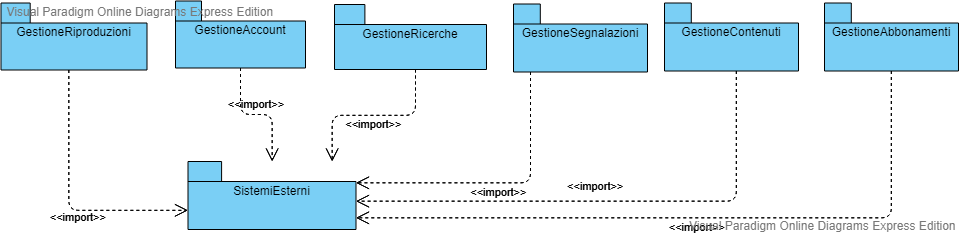
\includegraphics[width=14cm]{../Contents/Diagrams/Analisi/package/package_analisi.png}

\subsection{Diagrammi EBC}
Si utilizzano diagrammi EBC per meglio dettagliare l'analisi dell'architettura. I tre stereotipi dei diagrammi EBC sono:
\begin{itemize}
\item Entity: classe che mantiene informazioni di lunga duranta, tipicamente persistenti
\item Boundary: classe che modella l'interazione tra sistema e attori, spesso è un'astrazione di un elemento software di interfaccia
\item Control: classe che si occupa del controllo e coordinamento di altri oggetti, tipicamente è associabile a un caso d'uso
\end{itemize}
I diagrammi EBC sono riportati nella cartella ``Diagrams/Analisi/ebc". Per indicare una copia di uno stereotipo già presente in un certo diagramma, lo stereotipo viene mostrato in giallo, mentre la copia ``originale'' è mostrata in blu. 

\subsection{Diagrammi di Sequenza}
Sono stati usati i diagrammi di sequenza per l'analisi delle funzionalità. I diagrammi di sequenza ci permettono di visualizzare l'interazione tra le varie classi durante l'esecuzione di un caso d'uso. I diagrammi sono riportati nella cartella ``Diagrams/Analisi/sequence''.\\

\noindent{\large \textbf{Revisioni 10}} \\ \\
\begin{tabular}{|c | c | c | c|} 
 	\hline
	 Numero & Data & Descrizione \\ [0.5ex] 
	\hline\hline
	1 & 14/03/2020 & Stesura iniziale \\ 
	\hline
	2 & 09/04/2020 & Accorpamento di alcuni handler nei diagrammi EBC \\
	\hline
\end{tabular}